% generated by GAPDoc2LaTeX from XML source (Frank Luebeck)
\documentclass[a4paper,11pt]{report}

\usepackage{a4wide}
\sloppy
\pagestyle{myheadings}
\usepackage{amssymb}
\usepackage[latin1]{inputenc}
\usepackage{makeidx}
\makeindex
\usepackage{color}
\definecolor{FireBrick}{rgb}{0.5812,0.0074,0.0083}
\definecolor{RoyalBlue}{rgb}{0.0236,0.0894,0.6179}
\definecolor{RoyalGreen}{rgb}{0.0236,0.6179,0.0894}
\definecolor{RoyalRed}{rgb}{0.6179,0.0236,0.0894}
\definecolor{LightBlue}{rgb}{0.8544,0.9511,1.0000}
\definecolor{Black}{rgb}{0.0,0.0,0.0}

\definecolor{linkColor}{rgb}{0.0,0.0,0.554}
\definecolor{citeColor}{rgb}{0.0,0.0,0.554}
\definecolor{fileColor}{rgb}{0.0,0.0,0.554}
\definecolor{urlColor}{rgb}{0.0,0.0,0.554}
\definecolor{promptColor}{rgb}{0.0,0.0,0.589}
\definecolor{brkpromptColor}{rgb}{0.589,0.0,0.0}
\definecolor{gapinputColor}{rgb}{0.589,0.0,0.0}
\definecolor{gapoutputColor}{rgb}{0.0,0.0,0.0}

%%  for a long time these were red and blue by default,
%%  now black, but keep variables to overwrite
\definecolor{FuncColor}{rgb}{0.0,0.0,0.0}
%% strange name because of pdflatex bug:
\definecolor{Chapter }{rgb}{0.0,0.0,0.0}
\definecolor{DarkOlive}{rgb}{0.1047,0.2412,0.0064}


\usepackage{fancyvrb}

\usepackage{mathptmx,helvet}
\usepackage[T1]{fontenc}
\usepackage{textcomp}


\usepackage[
            pdftex=true,
            bookmarks=true,        
            a4paper=true,
            pdftitle={Written with GAPDoc},
            pdfcreator={LaTeX with hyperref package / GAPDoc},
            colorlinks=true,
            backref=page,
            breaklinks=true,
            linkcolor=linkColor,
            citecolor=citeColor,
            filecolor=fileColor,
            urlcolor=urlColor,
            pdfpagemode={UseNone}, 
           ]{hyperref}

\newcommand{\maintitlesize}{\fontsize{50}{55}\selectfont}

% write page numbers to a .pnr log file for online help
\newwrite\pagenrlog
\immediate\openout\pagenrlog =\jobname.pnr
\immediate\write\pagenrlog{PAGENRS := [}
\newcommand{\logpage}[1]{\protect\write\pagenrlog{#1, \thepage,}}
%% were never documented, give conflicts with some additional packages

\newcommand{\GAP}{\textsf{GAP}}

%% nicer description environments, allows long labels
\usepackage{enumitem}
\setdescription{style=nextline}

%% depth of toc
\setcounter{tocdepth}{1}



\usepackage[pdftex]{graphicx}

%% command for ColorPrompt style examples
\newcommand{\gapprompt}[1]{\color{promptColor}{\bfseries #1}}
\newcommand{\gapbrkprompt}[1]{\color{brkpromptColor}{\bfseries #1}}
\newcommand{\gapinput}[1]{\color{gapinputColor}{#1}}


\begin{document}

\logpage{[ 0, 0, 0 ]}
\begin{titlepage}
\mbox{}\vfill

\begin{center}{\maintitlesize \textbf{\textsf{SCSCP}\mbox{}}}\\
\vfill

\hypersetup{pdftitle=\textsf{SCSCP}}
\markright{\scriptsize \mbox{}\hfill \textsf{SCSCP} \hfill\mbox{}}
{\Huge \textbf{Symbolic Computation Software Composability Protocol\mbox{}}}\\
\vfill

{\Huge Version 2.1.2\mbox{}}\\[1cm]
{31 May 2012\mbox{}}\\[1cm]
\mbox{}\\[2cm]
{\Large \textbf{Alexander Konovalov    \mbox{}}}\\
{\Large \textbf{Steve Linton    \mbox{}}}\\
\hypersetup{pdfauthor=Alexander Konovalov    ; Steve Linton    }
\end{center}\vfill

\mbox{}\\
{\mbox{}\\
\small \noindent \textbf{Alexander Konovalov    }  Email: \href{mailto://alexk at mcs dot st-andrews dot ac dot uk} {\texttt{alexk at mcs dot st-andrews dot ac dot uk}}\\
  Homepage: \href{http://www.cs.st-andrews.ac.uk/~alexk/} {\texttt{http://www.cs.st-andrews.ac.uk/\texttt{\symbol{126}}alexk/}}\\
  Address: \begin{minipage}[t]{8cm}\noindent
 School of Computer Science\\
 University of St Andrews\\
 Jack Cole Building, North Haugh,\\
 St Andrews, Fife, KY16 9SX, Scotland \end{minipage}
}\\
{\mbox{}\\
\small \noindent \textbf{Steve Linton    }  Email: \href{mailto://sal at cs dot st-andrews dot ac dot uk} {\texttt{sal at cs dot st-andrews dot ac dot uk}}\\
  Homepage: \href{http://www.cs.st-andrews.ac.uk/~sal/} {\texttt{http://www.cs.st-andrews.ac.uk/\texttt{\symbol{126}}sal/}}\\
  Address: \begin{minipage}[t]{8cm}\noindent
 School of Computer Science\\
 University of St Andrews\\
 Jack Cole Building, North Haugh,\\
 St Andrews, Fife, KY16 9SX, Scotland \end{minipage}
}\\
\end{titlepage}

\newpage\setcounter{page}{2}
{\small 
\section*{Abstract}
\logpage{[ 0, 0, 1 ]}
 \index{SCSCP package@\textsf{SCSCP} package} The \textsf{GAP} package \textsf{SCSCP} implements the Symbolic Computation Software Composability protocol (\href{http://www.symbolic-computing.org/scscp} {\texttt{http://www.symbolic-computing.org/scscp}}) for the computational algebra system \textsf{GAP}. \mbox{}}\\[1cm]
{\small 
\section*{Copyright}
\logpage{[ 0, 0, 2 ]}
 {\copyright} 2007-2012 by Alexander Konovalov and Steve Linton

 \textsf{SCSCP} is free software; you can redistribute it and/or modify it under the terms of
the GNU General Public License as published by the Free Software Foundation;
either version 2 of the License, or (at your option) any later version. For
details, see the FSF's own site \href{http://www.gnu.org/licenses/gpl.html} {\texttt{http://www.gnu.org/licenses/gpl.html}}. 

 If you obtained \textsf{SCSCP}, we would be grateful for a short notification sent to one of the authors. 

 If you publish a result which was partially obtained with the usage of \textsf{SCSCP}, please cite it in the following form: 

 A. Konovalov and S. Linton. \emph{SCSCP --- Symbolic Computation Software Composability Protocol, Version 2.1.2;} 2012 (\href{http://www.cs.st-andrews.ac.uk/~alexk/scscp.htm} {\texttt{http://www.cs.st-andrews.ac.uk/\texttt{\symbol{126}}alexk/scscp.htm}}). \mbox{}}\\[1cm]
{\small 
\section*{Acknowledgements}
\logpage{[ 0, 0, 3 ]}
 The project 026133 "SCIEnce - Symbolic Computation Infrastructure for Europe"
(\href{http://www.symbolic-computing.org/} {\texttt{http://www.symbolic-computing.org/}}) is supported by the EU FP6 Programme. \mbox{}}\\[1cm]
{\small 
\section*{Colophon}
\logpage{[ 0, 0, 4 ]}
 Versions history: 
\begin{itemize}
\item Version 0.1 - first half of 2007;
\item Version 0.2 - December 2007;
\item Version 0.3 - May 2008;
\item Version 0.4 - August 2008;
\item Version 1.0 - March 2009;
\item Version 1.1 - May 2009;
\item Version 1.2 - March 2010.
\item Version 2.0 - October 2011.
\item Version 2.1 - March 2012.
\end{itemize}
 \mbox{}}\\[1cm]
\newpage

\def\contentsname{Contents\logpage{[ 0, 0, 5 ]}}

\tableofcontents
\newpage

 
\chapter{\textcolor{Chapter }{Preface}}\label{Preface}
\logpage{[ 1, 0, 0 ]}
\hyperdef{L}{X874E1D45845007FE}{}
{
  The \textsf{GAP} package \textsf{SCSCP} implements the Symbolic Computation Software Composability protocol \cite{SCSCP}. This protocol specifies an \textsf{OpenMath}-based remote procedure call framework, in which all messages (procedure calls
and returns of results of successful computation or error messages) are
encoded in \textsf{OpenMath} using content dictionaries \textsf{scscp1} and \textsf{scscp2} (\cite{scscp1cd}, \cite{scscp2cd}). Using the \textsf{SCSCP} package, \textsf{GAP} can communicate locally or remotely with any other \textsf{OpenMath}-enabled \textsf{SCSCP}-compliant application which may be not only another computer algebra system
but also another instance of the \textsf{GAP} system or even, for example, an external Java or C/C++ application via
libraries \href{http://java.symcomp.org/} {\texttt{http://java.symcomp.org/}} or \href{http://www.imcce.fr/Equipes/ASD/trip/scscp/} {\texttt{http://www.imcce.fr/Equipes/ASD/trip/scscp/}} providing an \textsf{SCSCP} API. Such communication will go into seamless manner for the \textsf{GAP} user, since all conversions from \textsf{GAP} to \textsf{OpenMath} and vice versa will be performed in the background. See the SCIEnce project
homepage \href{http://www.symbolic-computing.org/} {\texttt{http://www.symbolic-computing.org/}} for the details about computer algebra systems and other sotware supporting \textsf{SCSCP} 

 The \textsf{SCSCP} package for \textsf{GAP} has two main components: 
\begin{itemize}
\item SCSCP server;
\item SCSCP client.
\end{itemize}
 There are several ways to start \textsf{GAP} \textsf{SCSCP} server: 
\begin{itemize}
\item call \texttt{RunSCSCPserver} (\ref{RunSCSCPserver}) from the \textsf{GAP} session specifying the server name and the port number from the \textsf{GAP} session; 
\item start \textsf{GAP} as \texttt{gap myserver.g}, where \texttt{myserver.g} is the server configuration file with the last command being the call of \texttt{RunSCSCPserver} (\ref{RunSCSCPserver}) (an example of such configuration file is given in \texttt{scscp/example/myserver.g} ); 
\item start \textsf{GAP} as a daemon using the script \texttt{gapd.sh} which is supplied in the root directory of the package (for the description of
all available options see comments in \texttt{gapd.sh}). 
\end{itemize}
 During startup the server installs all procedures that it will provide and
loads their lookup mechanisms, and then begins to listen to the specified
port. The recommended port number is 26133 which has been assigned to SCSCP by
the Internet Assigned Numbers Authority (IANA) in November 2007, see \href{http://www.iana.org/assignments/port-numbers} {\texttt{http://www.iana.org/assignments/port-numbers}}. 

 When the server accepts a connection from client, it starts the
"accept-evaluate-return" loop: 
\begin{itemize}
\item accepts the \texttt{"procedure{\textunderscore}call";} message;
\item performs lookup of the appropriate GAP function;
\item evaluates the result (or produces a side-effect);
\item returns the result in the \texttt{"procedure{\textunderscore}completed"} message or returns an error in the \texttt{"procedure{\textunderscore}terminated"} message.
\end{itemize}
 The server works in a "multi-user" mode. When one client is connected, the
server is busy for other clients. As soon as the computation is finished and
the client is disconnected, the server is waiting for the next connection, and
normally it never stops until it will be terminated by the service provider.
The server maintain a queue of five incoming connections (this parameter can
be easily modified), and on each iteration evaluates the next request from the
queue. 

 There is an \textsf{SCSCP} server accessible at \texttt{chrystal.mcs.st-andrews.ac.uk}, port 26133. It is running under development versions of the \textsf{GAP} system and a selection of currently distributed packages. The reader is
encouraged to try to use examples from the manual to access this service,
replacing \texttt{"localhost"} by its address, where appropriate. Please report to Alexander Konovalov if you
will discover any bugs or if the server seems not available. 

 The SCSCP client: 
\begin{itemize}
\item establishes connection with the specified server at the specified port;
\item sends the \texttt{"procedure{\textunderscore}call"} message to the server;
\item waits for the result of the computation or returns to pick it up later;
\item fetches the response, extracting the result from the \texttt{"procedure{\textunderscore}completed"} message or entering the break loop in the case of the \texttt{"procedure{\textunderscore}terminated"} message. 
\end{itemize}
 On the top of this functionality we built a set of instructions for simple
parallel computations framework using the \textsf{SCSCP} protocol, which allows to send several procedure calls in parallel and then
collect all results or pick up the first available result, and implements the
master-worker skeleton. These tools are presented in the Chapter \ref{Parallel}. 

 The package also implements a new kind of \textsf{GAP} input-output streams, namely input-output TCP streams (see Chapter \ref{UsingStreams}), based on the functionality for TCP/IP protocol usage provided by the \textsf{GAP} package \textsf{IO}. Such streams may constitute an independent interest for adapting
streams-using \textsf{GAP} code to use streams across the network. 

 Finally, the manual describes how the communication by \textsf{SCSCP} goes between several instances of the \textsf{GAP} system, but the same behaviour is expected from any \textsf{SCSCP}-compliant application: the set of supported \textsf{OpenMath} symbols clearly will be different, but the rules of communication are
precisely specified in the \textsf{SCSCP} specification \cite{SCSCP}. See the homepage of the SCIEnce project \href{http://www.symbolic-computing.org/} {\texttt{http://www.symbolic-computing.org/}} for the information about \textsf{SCSCP}-compliant computer algebra systems and other tools developed in the project. }

 
\chapter{\textcolor{Chapter }{Installation}}\label{Intro}
\logpage{[ 2, 0, 0 ]}
\hyperdef{L}{X8360C04082558A12}{}
{
  
\section{\textcolor{Chapter }{Installation and system requirements}}\label{Install}
\logpage{[ 2, 1, 0 ]}
\hyperdef{L}{X7DB566D5785B7DBC}{}
{
  The \textsf{SCSCP} client for \textsf{GAP} is fully functional under \textsf{GAP} 4.4 and works in UNIX/Linux environments, Mac OS X (UNIX installation) and MS
Windows. 

 The \textsf{SCSCP} server for \textsf{GAP} works in UNIX/Linux environments and Mac OS X (UNIX installation), but does
not work under MS Windows. It is fully functional with the \textsf{GAP} development version and goes automatically into the compatibility mode to work
with \textsf{GAP} 4.4.12 and earlier versions. The only limitation of this compatibility mode is
that in the case of an error the break loop occurs on the server and can not
be transmitted to the client (however, if the service consumer is the service
provider himself/herself, then this is not as crucial as it might be in the
general case). After the \textsf{GAP} 4.5 release the package will fully be compatible with the official \textsf{GAP} releases. 

 To use the \textsf{SCSCP} package it is necessary to install recent versions of \textsf{GAP}4 packages \textsf{IO} \cite{IO}, \textsf{GAPDoc} \cite{GAPDoc} and \textsf{OpenMath} \cite{openmath}. 

 The \textsf{SCSCP} package is distributed in standard formats (\texttt{tar.gz}, \texttt{tar.bz2}) and can be obtained from \href{http://www.cs.st-andrews.ac.uk/~alexk/scscp.htm} {\texttt{http://www.cs.st-andrews.ac.uk/\texttt{\symbol{126}}alexk/scscp.htm}} or from the \textsf{GAP} web site (the latter also offers \texttt{zoo}- and \texttt{win.zip}-archives. To unpack the \texttt{zoo}-archive the program \texttt{unzoo} is needed, which can be obtained from the \textsf{GAP} homepage \href{http://www.gap-system.org/} {\texttt{http://www.gap-system.org/}} (see section `Distribution'). To install \textsf{SCSCP} package, put its \texttt{zoo}-archive into the \texttt{pkg} subdirectory of your \textsf{GAP}4.4 installation and enter the command \texttt{unzoo -x scscp-X.X.X.zoo}, then the subdirectory \texttt{scscp} (containing subdirectories \texttt{doc}, \texttt{lib} etc.) will be created in the \texttt{pkg} subdirectory. Installation using other archive formats is performed in a
similar way. 

 When there are no access rights to the root directory of the main \textsf{GAP} installation, it is also possible to install the package \emph{outside the \textsf{GAP} main directory} by unpacking it inside a directory \texttt{MYGAPDIR/pkg}. Then to load the package \textsf{GAP} should be started with \texttt{-l ";MYGAPDIR"} option. }

 
\section{\textcolor{Chapter }{Configuration files}}\label{Config}
\logpage{[ 2, 2, 0 ]}
\hyperdef{L}{X878084B083D5217F}{}
{
  There are four files in the package which may need to be modified to setup and
customise the package. The first three files are related with the server's
functionality: 
\begin{itemize}
\item  \texttt{scscp/config.g} specifies: 
\begin{itemize}
\item  default \texttt{InfoLevel} for the \texttt{InfoSCSCP} (\ref{InfoSCSCP}) class; 
\item  default \textsf{SCSCP} server name and port to be used by \texttt{RunSCSCPserver} (\ref{RunSCSCPserver}) if \textsf{GAP} is started with the \texttt{scscp/example/myserver.g} file; 
\item  whether the server accepts calls to procedures which are standard \textsf{OpenMath} symbols, or only procedures installed in the transient content dictionary (see \texttt{InstallSCSCPprocedure} (\ref{InstallSCSCPprocedure})); 
\item  service description to be returned to the client by \texttt{GetServiceDescription} (\ref{GetServiceDescription}). 
\end{itemize}
 
\item  \texttt{scscp/gapd.sh} is the script to start the \textsf{GAP} \textsf{SCSCP} server as a daemon. To use it, adjust the local call of \textsf{GAP} and, if necessary, call options (for example, memory usage, startup from the
workspace etc.) and the location of the root directory of the \textsf{SCSCP} package in section 1 of this script. 
\item  \texttt{scscp/example/myserver.g} is an example of the server configuration file which loads all necessary
packages, reads all needed code, installs all procedures which will be exposed
to the client and finally starts the \textsf{SCSCP} server (see Chapter \ref{Server}). 
\end{itemize}
 The fourth file is related with the client's functionality for parallel
computations: 
\begin{itemize}
\item  The file \texttt{scscp/configpar.g} assigns the global variable \texttt{SCSCPservers} which specifies a list of hosts and ports to search for \textsf{SCSCP} services (which may be not only represented by \textsf{GAP} services, but also by another \textsf{SCSCP}-compliant systems). It will be used to run parallel computations with the \textsf{SCSCP} package (see Chapter \ref{Parallel}). 
\end{itemize}
 See comments in these configuration files for further details and examples. }

 }

 
\chapter{\textcolor{Chapter }{Using streams}}\label{UsingStreams}
\logpage{[ 3, 0, 0 ]}
\hyperdef{L}{X7CB06121820FD0DD}{}
{
  The package implements new kind of \textsf{GAP} input-output streams, called input-output TCP streams. Such streams are based
on the functionality for the TCP/IP protocol usage provided by the \textsf{GAP} package \textsf{IO}, and may constitute an independent interest for \textsf{GAP} users. 

 Input-output TCP streams are intended to support all operations, implemented
for streams in \textsf{GAP}. It is assumed that all existing code using streams should work with this
kind of streams as well (please let us know, if you will notice that this is
not the case!). We installed methods for input-output TCP streams to support
the following operations: \texttt{ViewObj} (\textbf{Reference: ViewObj}), \texttt{PrintObj} (\textbf{Reference: PrintObj}), \texttt{ReadByte} (\textbf{Reference: ReadByte}), \texttt{ReadLine} (\textbf{Reference: ReadLine}), \texttt{ReadAll} (\textbf{Reference: ReadAll}), \texttt{WriteByte} (\textbf{Reference: WriteByte}), \texttt{WriteLine} (\textbf{Reference: WriteLine}), \texttt{WriteAll} (\textbf{Reference: WriteAll}), \texttt{IsEndOfStream} (\textbf{Reference: IsEndOfStream}), \texttt{CloseStream} (\textbf{Reference: CloseStream}), \texttt{FileDescriptorOfStream} (\textbf{Reference: FileDescriptorOfStream}), \texttt{UNIXSelect} (\textbf{Reference: UNIXSelect}). 

 
\section{\textcolor{Chapter }{Input-output TCP streams}}\label{Streams}
\logpage{[ 3, 1, 0 ]}
\hyperdef{L}{X79EB93A27D9AC115}{}
{
  

\subsection{\textcolor{Chapter }{IsInputOutputTCPStream}}
\logpage{[ 3, 1, 1 ]}\nobreak
\hyperdef{L}{X805BB9468642A787}{}
{\noindent\textcolor{FuncColor}{$\triangleright$\ \ \texttt{IsInputOutputTCPStream\index{IsInputOutputTCPStream@\texttt{IsInputOutputTCPStream}}
\label{IsInputOutputTCPStream}
}\hfill{\scriptsize (filter)}}\\


 \texttt{IsInputOutputTCPStream} is a subcategory of \texttt{IsInputOutputStream} (\textbf{Reference: IsInputOutputStream}). Streams in the category \texttt{IsInputOutputTCPStream} are created with the help of the function \texttt{InputOutputTCPStream} (\ref{InputOutputTCPStream:for client}) with one or two arguments dependently on whether they will be used in the
client or server mode. Examples of their creation and usage will be given in
subsequent sections. }

 

\subsection{\textcolor{Chapter }{IsInputOutputTCPStreamRep}}
\logpage{[ 3, 1, 2 ]}\nobreak
\hyperdef{L}{X817A945B83659813}{}
{\noindent\textcolor{FuncColor}{$\triangleright$\ \ \texttt{IsInputOutputTCPStreamRep\index{IsInputOutputTCPStreamRep@\texttt{IsInputOutputTCPStreamRep}}
\label{IsInputOutputTCPStreamRep}
}\hfill{\scriptsize (filter)}}\\


 This is the representation used for streams in the category \texttt{IsInputOutputTCPStream} (\ref{IsInputOutputTCPStream}). }

 

\subsection{\textcolor{Chapter }{InputOutputTCPStream (for server)}}
\logpage{[ 3, 1, 3 ]}\nobreak
\hyperdef{L}{X7E3D43CF7B049F04}{}
{\noindent\textcolor{FuncColor}{$\triangleright$\ \ \texttt{InputOutputTCPStream({\mdseries\slshape desc})\index{InputOutputTCPStream@\texttt{InputOutputTCPStream}!for server}
\label{InputOutputTCPStream:for server}
}\hfill{\scriptsize (function)}}\\
\noindent\textcolor{FuncColor}{$\triangleright$\ \ \texttt{InputOutputTCPStream({\mdseries\slshape host, port})\index{InputOutputTCPStream@\texttt{InputOutputTCPStream}!for client}
\label{InputOutputTCPStream:for client}
}\hfill{\scriptsize (function)}}\\
\textbf{\indent Returns:\ }
 stream 



 The one-argument version must be called from the \textsf{SCSCP} server. Its argument \mbox{\texttt{\mdseries\slshape desc}} must be a socket descriptor obtained using \texttt{IO{\textunderscore}accept} (\textbf{IO: IO{\textunderscore}accept}) function from the \textsf{IO} package (see the example below). It returns a stream in the category \texttt{IsInputOutputTCPStream} (\ref{IsInputOutputTCPStream}) which will use this socket to accept incoming connections. In most cases, the
one-argument version is called automatically from \texttt{RunSCSCPserver} (\ref{RunSCSCPserver}) rather then manually. 

 The version with two arguments, a string \mbox{\texttt{\mdseries\slshape host}} and an integer \mbox{\texttt{\mdseries\slshape port}}, must be called from the \textsf{SCSCP} client. It returns a stream in the category \texttt{IsInputOutputTCPStream} (\ref{IsInputOutputTCPStream}) which will be used by the client for communication with the \textsf{SCSCP} server running at hostname \mbox{\texttt{\mdseries\slshape host}} on port \mbox{\texttt{\mdseries\slshape port}}. In most cases, the two-argument version is called automatically from the
higher level functions, for example, \texttt{EvaluateBySCSCP} (\ref{EvaluateBySCSCP}). }

 }

 
\section{\textcolor{Chapter }{Example of client-server communication via input-output TCP streams}}\label{StreamsExample}
\logpage{[ 3, 2, 0 ]}
\hyperdef{L}{X86CA5D6C79B32600}{}
{
  The following example demonstrates the low-level interaction between client
and server using input-output TCP stream, and shows how such streams are
created in the function \texttt{RunSCSCPserver} (\ref{RunSCSCPserver}). It uses some functions from the \textsf{IO} package (see the \textsf{IO} manual for their description). We will show step by step what is happens on
server and client (of course, if you will try this example, the numbers
denoting descriptors may be different). 

 Firts, we will start two \textsf{GAP} sessions, one for the server, another one for the client. Now we enter the
following commands on the server's side: 
\begin{Verbatim}[commandchars=!@|,fontsize=\small,frame=single,label=Example]
  
  !gapprompt@gap>| !gapinput@sock := IO_socket( IO.PF_INET, IO.SOCK_STREAM, "tcp" );|
  3
  !gapprompt@gap>| !gapinput@lookup := IO_gethostbyname( "localhost" );|
  rec( name := "localhost", aliases := [  ], addrtype := 2, length := 4, 
    addr := [ "\177\000\000\>" ] )
  !gapprompt@gap>| !gapinput@port:=26133;|
  26133
  !gapprompt@gap>| !gapinput@res := IO_bind( sock, IO_make_sockaddr_in( lookup.addr[1], port ) );|
  true
  !gapprompt@gap>| !gapinput@IO_listen( sock, 5 );|
  true
  !gapprompt@gap>| !gapinput@socket_descriptor := IO_accept( sock, IO_MakeIPAddressPort("0.0.0.0",0) );|
  
\end{Verbatim}
 After the last command you will not see the \textsf{GAP} prompt because the server starts to wait for an incoming connection. Now we go
to the client's side and create an input-output TCP stream to the server. Here
it can be created in one step: 
\begin{Verbatim}[commandchars=!@|,fontsize=\small,frame=single,label=Example]
  
  !gapprompt@gap>| !gapinput@clientstream:=InputOutputTCPStream( "localhost", 26133 );|
  Creating a socket...
  Connecting to a remote socket via TCP/IP...
  
\end{Verbatim}
 Now we are trying to connect to the server, and as soon as the connection will
be established, the stream will be created at the client side, and we will see
the output and the new \textsf{GAP} prompt: 
\begin{Verbatim}[commandchars=!@|,fontsize=\small,frame=single,label=Example]
  
  < input/output TCP stream to localhost >
  gap>
  
\end{Verbatim}
 On the server you will get the socket descriptor and then you will be able to
create a stream from it: 
\begin{Verbatim}[commandchars=!@|,fontsize=\small,frame=single,label=Example]
  
  4
  !gapprompt@gap>| !gapinput@serverstream := InputOutputTCPStream( socket_descriptor );|
  < input/output TCP stream to socket >
  
\end{Verbatim}
 Now we can write to this stream on the client side and then read from it on
the server side and backwards. First, write on the client: 
\begin{Verbatim}[commandchars=!@|,fontsize=\small,frame=single,label=Example]
  
  !gapprompt@gap>| !gapinput@WriteLine( clientstream, "12345" );|
  true
  
\end{Verbatim}
 Now read and write on the server: 
\begin{Verbatim}[commandchars=!@|,fontsize=\small,frame=single,label=Example]
  
  !gapprompt@gap>| !gapinput@ReadLine( serverstream );|
  "12345\n"
  !gapprompt@gap>| !gapinput@WriteLine( serverstream, "54321" );|
  true
  
\end{Verbatim}
 And finally we read on the client and close the stream: 
\begin{Verbatim}[commandchars=!@|,fontsize=\small,frame=single,label=Example]
  
  !gapprompt@gap>| !gapinput@ReadLine( clientstream );|
  "54321\n"
  !gapprompt@gap>| !gapinput@CloseStream( clientstream );|
  
\end{Verbatim}
 and similarly close the stream on the server: 
\begin{Verbatim}[commandchars=!@|,fontsize=\small,frame=single,label=Example]
  
  !gapprompt@gap>| !gapinput@CloseStream( serverstream );|
  
\end{Verbatim}
 In this way one can organise remote communication between two copies of \textsf{GAP} in various ways. In subsequent chapters we explain how it is implemented using \textsf{SCSCP} to ensure compatibility not only with \textsf{GAP} but with any other \textsf{SCSCP}-compliant system. }

 }

 
\chapter{\textcolor{Chapter }{Message exchange by \textsf{SCSCP}}}\label{SCSCPmessages}
\logpage{[ 4, 0, 0 ]}
\hyperdef{L}{X79B21F427ECE8C38}{}
{
  To ensure the message exchange as required by \textsf{SCSCP} specification, the \textsf{SCSCP} package extends the global record \texttt{OMsymRecord} from the \textsf{OpenMath} package with new entries to support \textsf{scscp1} and \textsf{scscp2} content dictionaries (\cite{scscp1cd}, \cite{scscp2cd}), and also service-dependent transient private content dictionaries (see
Chapter \ref{Server} for details about transient content dictionaries). It also overwrites some \textsf{OpenMath} functions by their extended (but backwards compatible) versions, and adds some
new \textsf{OpenMath}-related functions to send and receive \textsf{SCSCP} messages, documented below. 

 Note that functions documented in this chapter belong to the middle-level
interface, and the user may find it more convenient to use functions developed
on top of them and explained in next chapters. 
\section{\textcolor{Chapter }{Communication with the \textsf{SCSCP} server}}\label{SCSCPclient}
\logpage{[ 4, 1, 0 ]}
\hyperdef{L}{X8355ECDA7D5B1331}{}
{
  

\subsection{\textcolor{Chapter }{StartSCSCPsession}}
\logpage{[ 4, 1, 1 ]}\nobreak
\hyperdef{L}{X86D913277AFF2366}{}
{\noindent\textcolor{FuncColor}{$\triangleright$\ \ \texttt{StartSCSCPsession({\mdseries\slshape stream})\index{StartSCSCPsession@\texttt{StartSCSCPsession}}
\label{StartSCSCPsession}
}\hfill{\scriptsize (function)}}\\
\textbf{\indent Returns:\ }
 string 



 Initialises \textsf{SCSCP} session and negotiates with the server about the version of the protocol.
Returns the string with the \texttt{service{\textunderscore}id} (which may be used later as a part of the call identifier) or causes an error
message if can not perform these tasks. 
\begin{Verbatim}[commandchars=!@|,fontsize=\small,frame=single,label=Example]
  
  !gapprompt@gap>| !gapinput@s := InputOutputTCPStream("localhost",26133);|
  < input/output TCP stream to localhost:26133 >
  !gapprompt@gap>| !gapinput@StartSCSCPsession(s);|
  "localhost:26133:5541"
  !gapprompt@gap>| !gapinput@CloseStream( s );|
  
\end{Verbatim}
 After the call to \texttt{StartSCSCPsession} the \textsf{SCSCP} server is ready to accept procedure calls. }

 

\subsection{\textcolor{Chapter }{OMPutProcedureCall}}
\logpage{[ 4, 1, 2 ]}\nobreak
\hyperdef{L}{X81EC8AAA78F62CB7}{}
{\noindent\textcolor{FuncColor}{$\triangleright$\ \ \texttt{OMPutProcedureCall({\mdseries\slshape stream, proc{\textunderscore}name, objrec})\index{OMPutProcedureCall@\texttt{OMPutProcedureCall}}
\label{OMPutProcedureCall}
}\hfill{\scriptsize (function)}}\\
\textbf{\indent Returns:\ }
 nothing 



 Takes a stream \mbox{\texttt{\mdseries\slshape stream}}, the string \mbox{\texttt{\mdseries\slshape proc{\textunderscore}name}} and a record \mbox{\texttt{\mdseries\slshape objrec}}, and writes to \mbox{\texttt{\mdseries\slshape stream}} an \textsf{OpenMath} object \texttt{procedure{\textunderscore}call} for the procedure \mbox{\texttt{\mdseries\slshape proc{\textunderscore}name}} with arguments given by the list \texttt{objrec.object} and procedure call options (which should be encoded as \textsf{OpenMath} attributes) given in the list \texttt{objrec.attributes}. 

 This function accepts options \texttt{cd} and \texttt{debuglevel}. 

 \texttt{cd:="cdname"} may be used to specify the name of the content dictionary if the procedure is
actually a standard \textsf{OpenMath} symbol. Note that the server may reject such a call if it accepts only calls
of procedures from the transient content dictionary, see \texttt{InstallSCSCPprocedure} (\ref{InstallSCSCPprocedure}) for explanation). If the \texttt{cdname} is not specified, \texttt{scscp{\textunderscore}transient{\textunderscore}1} content dictionary will be assumed by default. The value of the \texttt{debuglevel} option is an integer. If it is non-zero, the \texttt{procedure{\textunderscore}completed} message will carry on also some additional information about the call, for
example, runtime and memory used.  
\begin{Verbatim}[commandchars=!@|,fontsize=\small,frame=single,label=Example]
  
  !gapprompt@gap>| !gapinput@t:="";; stream:=OutputTextString(t,true);;|
  !gapprompt@gap>| !gapinput@OMPutProcedureCall( stream, "WS_Factorial", rec( object:= [ 5 ], |
  !gapprompt@>| !gapinput@     attributes:=[ [ "call_id", "user007" ], |
  !gapprompt@>| !gapinput@                   ["option_runtime",1000],|
  !gapprompt@>| !gapinput@                   ["option_min_memory",1024], |
  !gapprompt@>| !gapinput@                   ["option_max_memory",2048],|
  !gapprompt@>| !gapinput@                   ["option_debuglevel",1], |
  !gapprompt@>| !gapinput@                   ["option_return_object"] ] ) );;|
  !gapprompt@gap>| !gapinput@Print(t);|
  <?scscp start ?>
  <OMOBJ>
  	<OMATTR>
  		<OMATP>
  			<OMS cd="scscp1" name="call_id"/>
  			<OMSTR>user007</OMSTR>
  			<OMS cd="scscp1" name="option_runtime"/>
  			<OMI>1000</OMI>
  			<OMS cd="scscp1" name="option_min_memory"/>
  			<OMI>1024</OMI>
  			<OMS cd="scscp1" name="option_max_memory"/>
  			<OMI>2048</OMI>
  			<OMS cd="scscp1" name="option_debuglevel"/>
  			<OMI>1</OMI>
  			<OMS cd="scscp1" name="option_return_object"/>
  			<OMSTR></OMSTR>
  		</OMATP>
  		<OMA>
  			<OMS cd="scscp1" name="procedure_call"/>
  			<OMA>
  				<OMS cd="scscp_transient_1" name="WS_Factorial"/>
  				<OMI>5</OMI>
  			</OMA>
  		</OMA>
  	</OMATTR>
  </OMOBJ>
  <?scscp end ?>
  
\end{Verbatim}
 }

 

\subsection{\textcolor{Chapter }{SCSCPwait}}
\logpage{[ 4, 1, 3 ]}\nobreak
\hyperdef{L}{X7ABD2EA6792279CF}{}
{\noindent\textcolor{FuncColor}{$\triangleright$\ \ \texttt{SCSCPwait({\mdseries\slshape stream[, timeout]})\index{SCSCPwait@\texttt{SCSCPwait}}
\label{SCSCPwait}
}\hfill{\scriptsize (function)}}\\
\textbf{\indent Returns:\ }
 nothing 



 This function may be used by the \textsf{SCSCP} client to wait (using \texttt{IO{\textunderscore}select} (\textbf{IO: IO{\textunderscore}select})) until the result of the procedure call will be available from \mbox{\texttt{\mdseries\slshape stream}}. By default the timeout is one hour, to specify another value give it as the
optional second argument in seconds. See the end of this chapter for the
example. }

 

\subsection{\textcolor{Chapter }{OMGetObjectWithAttributes}}
\logpage{[ 4, 1, 4 ]}\nobreak
\hyperdef{L}{X7E0FE0CF7DD2E00F}{}
{\noindent\textcolor{FuncColor}{$\triangleright$\ \ \texttt{OMGetObjectWithAttributes({\mdseries\slshape stream})\index{OMGetObjectWithAttributes@\texttt{OMGetObjectWithAttributes}}
\label{OMGetObjectWithAttributes}
}\hfill{\scriptsize (function)}}\\
\textbf{\indent Returns:\ }
 record with components \texttt{object} and \texttt{attributes}, or \texttt{fail} 



  This function is similar to the function \texttt{OMGetObject} from the \textsf{OpenMath} package, and the main difference is that it is able to understand \textsf{OpenMath} attribution pairs. It retrieves exactly one \textsf{OpenMath} object from the stream \mbox{\texttt{\mdseries\slshape stream}}, and stores it in the \texttt{object} component of the returned record. If the \textsf{OpenMath} object has no attributes, the \texttt{attributes} component of the returned record will be an empty list, otherwise it will
contain pairs \texttt{[attribute{\textunderscore}name,attribute{\textunderscore}value]}, where \texttt{attribute{\textunderscore}name} is a string, and \texttt{attribute{\textunderscore}value} is a \textsf{GAP} object, whose type is determined by the kind of an attribute. Only attributes,
defined by the SCSCP are allowed, otherwise an error message will be
displayed. 

 If the procedure was not successful, the function returns \texttt{fail} instead of an error message like the function \texttt{OMGetObject} (\textbf{OpenMath: OMGetObject}) does. Returning \texttt{fail} is useful when \texttt{OMGetObjectWithAttributes} is used inside accept-evaluate-return loop. 

 As an example, the file \texttt{scscp/tst/omdemo.om} contains some \textsf{OpenMath} objects, including those from the SCSCP Specification \cite{SCSCP}. We can retrieve them from this file, preliminary installing some SCSCP
procedures using the function \texttt{InstallSCSCPprocedure} (\ref{InstallSCSCPprocedure}): 
\begin{Verbatim}[commandchars=!@|,fontsize=\small,frame=single,label=Example]
  
  !gapprompt@gap>| !gapinput@InstallSCSCPprocedure("WS_Factorial", Factorial );|
  !gapprompt@gap>| !gapinput@InstallSCSCPprocedure("GroupIdentificationService", IdGroup );|
  !gapprompt@gap>| !gapinput@InstallSCSCPprocedure("GroupByIdNumber", SmallGroup );|
  !gapprompt@gap>| !gapinput@InstallSCSCPprocedure( "Length", Length, 1, 1 );|
  !gapprompt@gap>| !gapinput@test:=Filename( Directory( Concatenation(|
  !gapprompt@>| !gapinput@        GAPInfo.PackagesInfo.("scscp")[1].InstallationPath,"/tst/" ) ), |
  !gapprompt@>| !gapinput@        "omdemo.om" );;|
  !gapprompt@gap>| !gapinput@stream:=InputTextFile(test);;|
  !gapprompt@gap>| !gapinput@OMGetObjectWithAttributes(stream); |
  rec( 
    attributes := [ [ "option_return_object", "" ], [ "call_id", "5rc6rtG62" ] ]
      , object := 6 )
  !gapprompt@gap>| !gapinput@OMGetObjectWithAttributes(stream);|
  rec( attributes := [  ], object := 1 )
  !gapprompt@gap>| !gapinput@OMGetObjectWithAttributes(stream);|
  rec( attributes := [  ], object := 120 )
  !gapprompt@gap>| !gapinput@OMGetObjectWithAttributes(stream);|
  rec( 
    attributes := [ [ "call_id", "alexk_9053" ], [ "option_runtime", 300000 ], 
        [ "option_min_memory", 40964 ], [ "option_max_memory", 134217728 ], 
        [ "option_debuglevel", 2 ], [ "option_return_object", "" ] ],
    object := [ 24, 12 ] )
  !gapprompt@gap>| !gapinput@OMGetObjectWithAttributes(stream);|
  rec( 
    attributes := [ [ "call_id", "alexk_9053" ], [ "option_return_cookie", "" ] 
       ], object := <pc group of size 24 with 4 generators> )
  !gapprompt@gap>| !gapinput@OMGetObjectWithAttributes(stream);|
  rec( attributes := [ [ "call_id", "alexk_9053" ], [ "info_runtime", 1234 ], 
        [ "info_memory", 134217728 ] ], object := [ 24, 12 ] )
  !gapprompt@gap>| !gapinput@CloseStream( stream );|
  
\end{Verbatim}
 }

 }

 
\section{\textcolor{Chapter }{Communication with the \textsf{SCSCP} client}}\label{SCSCPserver}
\logpage{[ 4, 2, 0 ]}
\hyperdef{L}{X7A8771C084107E79}{}
{
  

\subsection{\textcolor{Chapter }{OMPutProcedureCompleted}}
\logpage{[ 4, 2, 1 ]}\nobreak
\hyperdef{L}{X7C5C23A47A86EAEC}{}
{\noindent\textcolor{FuncColor}{$\triangleright$\ \ \texttt{OMPutProcedureCompleted({\mdseries\slshape stream, objrec})\index{OMPutProcedureCompleted@\texttt{OMPutProcedureCompleted}}
\label{OMPutProcedureCompleted}
}\hfill{\scriptsize (function)}}\\
\textbf{\indent Returns:\ }
 \texttt{true} 



 Takes a stream \mbox{\texttt{\mdseries\slshape stream}}, and a record \mbox{\texttt{\mdseries\slshape objrec}}, and writes to \mbox{\texttt{\mdseries\slshape stream}} an \textsf{OpenMath} object \texttt{procedure{\textunderscore}completed} with the result being \texttt{objrec.object} and information messages (as \textsf{OpenMath} attributes) given in the list \texttt{objrec.attributes}. 
\begin{Verbatim}[commandchars=!@|,fontsize=\small,frame=single,label=Example]
  
  !gapprompt@gap>| !gapinput@t:="";; stream:=OutputTextString(t,true);;|
  !gapprompt@gap>| !gapinput@OMPutProcedureCompleted( stream, |
  !gapprompt@>| !gapinput@     rec(object:=120, |
  !gapprompt@>| !gapinput@     attributes:=[ [ "call_id", "user007" ] ] ) );|
  true
  !gapprompt@gap>| !gapinput@Print(t);|
  <?scscp start ?>
  <OMOBJ>
  	<OMATTR>
  		<OMATP>
  			<OMS cd="scscp1" name="call_id"/>
  			<OMSTR>user007</OMSTR>
  		</OMATP>
  		<OMA>
  			<OMS cd="scscp1" name="procedure_completed"/>
  			<OMI>120</OMI>
  		</OMA>
  	</OMATTR>
  </OMOBJ>
  <?scscp end ?>
  
\end{Verbatim}
 }

 

\subsection{\textcolor{Chapter }{OMPutProcedureTerminated}}
\logpage{[ 4, 2, 2 ]}\nobreak
\hyperdef{L}{X7FB47E3E86C7C9F9}{}
{\noindent\textcolor{FuncColor}{$\triangleright$\ \ \texttt{OMPutProcedureTerminated({\mdseries\slshape stream, objrec, error{\textunderscore}cd, error{\textunderscore}type})\index{OMPutProcedureTerminated@\texttt{OMPutProcedureTerminated}}
\label{OMPutProcedureTerminated}
}\hfill{\scriptsize (function)}}\\
\textbf{\indent Returns:\ }
 nothing 



 Takes a stream \mbox{\texttt{\mdseries\slshape stream}}, and a record with an error message \mbox{\texttt{\mdseries\slshape objrec}} (for example \texttt{rec( attributes := [ [ "call{\textunderscore}id",
"localhost:26133:87643:gcX33cCf" ] ],} \texttt{object := "localhost:26133 reports : Rational operations:
{\textless}divisor{\textgreater} must not be zero")} and writes to the \mbox{\texttt{\mdseries\slshape stream}} an \textsf{OpenMath} object \texttt{procedure{\textunderscore}terminated} containing an error determined by the symbol \mbox{\texttt{\mdseries\slshape error{\textunderscore}type}} from the content dictionary \mbox{\texttt{\mdseries\slshape error{\textunderscore}cd}} (for example, \texttt{error{\textunderscore}memory}, \texttt{error{\textunderscore}runtime} or \texttt{error{\textunderscore}system{\textunderscore}specific} from the \textsf{scscp1} content dictionary (\cite{scscp1cd}). 

 This is the internal function of the package which is used only in the code
for the \textsf{SCSCP} server to return the error message to the client. }

 }

 
\section{\textcolor{Chapter }{Example: \textsf{SCSCP} session}}\label{SCSCPsession}
\logpage{[ 4, 3, 0 ]}
\hyperdef{L}{X845ACA2578B2D808}{}
{
  In the following example we start an \textsf{SCSCP} session and perform ten procedure calls in a loop before closing that session.
Note that we demonstrate the usage of the session ID \texttt{sid} and the function \texttt{RandomString} from the \textsf{OpenMath} package to produce some unique call identifier. The call ID is a mandatory
attribute for any procedure call, however, it is not nesessarily random; for
example, it may be just a string with the number of the procedure call. 
\begin{Verbatim}[commandchars=!@|,fontsize=\small,frame=single,label=Example]
  
  !gapprompt@gap>| !gapinput@stream:=InputOutputTCPStream( "localhost", 26133 );|
  < input/output TCP stream to localhost:26133 >
  !gapprompt@gap>| !gapinput@sid := StartSCSCPsession( stream );|
  "localhost:26133:5541"
  !gapprompt@gap>| !gapinput@res:=[];|
  [  ]
  !gapprompt@gap>| !gapinput@for i in [1..10] do|
  !gapprompt@>| !gapinput@    OMPutProcedureCall( stream, "WS_Factorial", |
  !gapprompt@>| !gapinput@      rec( object := [ i ], |
  !gapprompt@>| !gapinput@       attributes := [ [ "call_id", |
  !gapprompt@>| !gapinput@         Concatenation( sid, ":", RandomString(8) ) ] ] ) );|
  !gapprompt@>| !gapinput@    SCSCPwait( stream );|
  !gapprompt@>| !gapinput@    res[i]:=OMGetObjectWithAttributes( stream ).object;|
  !gapprompt@>| !gapinput@od;|
  !gapprompt@gap>| !gapinput@CloseStream(stream);|
  !gapprompt@gap>| !gapinput@res;|
  [ 1, 2, 6, 24, 120, 720, 5040, 40320, 362880, 3628800 ]
  
\end{Verbatim}
 Also note the usage of \texttt{SCSCPwait} (\ref{SCSCPwait}) to wait until the result of the computation will be available from \texttt{stream}. 

 In this example we assumed that there is an \textsf{SCSCP} server running at \texttt{localhost}, port 26133. In the next chapter we will explain how to configure and run a \textsf{GAP} \textsf{SCSCP} server and how to interrogate it from a \textsf{GAP} client to learn about its functionality. After that, we will proceed with the \textsf{SCSCP} client functionality for the end-user. }

 }

 
\chapter{\textcolor{Chapter }{Running SCSCP server}}\label{Server}
\logpage{[ 5, 0, 0 ]}
\hyperdef{L}{X7DEE95317812A998}{}
{
  
\section{\textcolor{Chapter }{Installation of \textsf{SCSCP} procedures}}\label{InstallProcedures}
\logpage{[ 5, 1, 0 ]}
\hyperdef{L}{X83F4F28486E2A9AF}{}
{
  There may various ways to run \textsf{SCSCP} server, for example: 
\begin{itemize}
\item  allowing generic services like evaluation of arbitrary \textsf{OpenMath} code; 
\item  offering highly specialized procedures like identification of groups of order
512; 
\item  providing access to a database of mathematical objects. 
\end{itemize}
 Each of these use cases requires certain control over the level of
functionality exposed to the client. To achieve this, before starting \textsf{SCSCP} service its provider must call the function \texttt{InstallSCSCPprocedure} (\ref{InstallSCSCPprocedure}) to make required procedures ``visible'' for the client. 

 Additionally, the service can be made made accessible only for clients running
on the same computer, or accessible only through a particular network
interface, or generally accessible. This customization is made at the stage of
starting the \textsf{SCSCP} server with the function \texttt{RunSCSCPserver} (\ref{RunSCSCPserver}). 

\subsection{\textcolor{Chapter }{InstallSCSCPprocedure}}
\logpage{[ 5, 1, 1 ]}\nobreak
\hyperdef{L}{X8031C2F4787E0C1A}{}
{\noindent\textcolor{FuncColor}{$\triangleright$\ \ \texttt{InstallSCSCPprocedure({\mdseries\slshape procname, procfunc[, description][, narg1[, narg2][, signature]]})\index{InstallSCSCPprocedure@\texttt{InstallSCSCPprocedure}}
\label{InstallSCSCPprocedure}
}\hfill{\scriptsize (function)}}\\
\textbf{\indent Returns:\ }
 nothing 



 For a string \mbox{\texttt{\mdseries\slshape procname}} and a function \mbox{\texttt{\mdseries\slshape procfunc}}, \texttt{InstallSCSCPprocedure} makes the \mbox{\texttt{\mdseries\slshape procfunc}} available as SCSCP procedure under the name \mbox{\texttt{\mdseries\slshape procname}}, adding it to the transient \textsf{OpenMath} content dictionary \texttt{scscp{\textunderscore}transient{\textunderscore}1} that will exist during the service lifetime. 

 The second argument \mbox{\texttt{\mdseries\slshape procfunc}} may be either a standard or user-defined \textsf{GAP} function (procedure, operation, etc.). 

 The rest of arguments are optional and may be used in a number of
combinations: 
\begin{itemize}
\item  \mbox{\texttt{\mdseries\slshape description}} is a string with the description of the procedure. It may be used by the help
system. If it is omitted, the procedure will be reported as undocumented. 
\item  \mbox{\texttt{\mdseries\slshape narg1}} is a non-negative integer, specifying the minimal number of arguments, and \mbox{\texttt{\mdseries\slshape narg2}} is a non-negative integer or infinity, specifying the maximal number of
arguments. If \mbox{\texttt{\mdseries\slshape narg2}} is omitted then the maximal number of arguments will be set to \mbox{\texttt{\mdseries\slshape narg1}}. If both \mbox{\texttt{\mdseries\slshape narg1}} and \mbox{\texttt{\mdseries\slshape narg2}} are omitted then the minimal number of arguments will be set to zero and their
maximal number will be set to infinity. 
\item  \mbox{\texttt{\mdseries\slshape signature}} is the signature record of the procedure. If the \mbox{\texttt{\mdseries\slshape signature}} is given, then the number of arguments must be explicitly specified (by \mbox{\texttt{\mdseries\slshape narg1}} with or without \mbox{\texttt{\mdseries\slshape narg2}}) at least to zero and infinity respectively (to ensure proper matching of
arguments). Note that it is completely acceptable for a symbol from a
transient content dictionary to overstate the set of symbols which may occur
in its children using the \texttt{scscp2.symbol{\textunderscore}set{\textunderscore}all} symbol, and to use standard \textsf{OpenMath} errors to reject requests later at the stage of their evaluation. For example,
using such approach, we will define the procedure \texttt{WS{\textunderscore}Factorial} accepting not only immediate \texttt{{\textless}OMI{\textgreater}} objects but anything which could be evaluated to an integer. 

. The signature must be either a list of records, where $i$-th record corresponds to the $i$-th argument, or a record itself meaning that it specifies the signature for
all arguments. In the latter case the record may be \texttt{rec( )} corresponding to the \texttt{scscp2.symbol{\textunderscore}set{\textunderscore}all} symbol (this will be assumed by default if the signature will be omitted). 

 If more detailed description of allowed arguments is needed, the signature
record (one for all arguments or a specific one) may have components \texttt{CDgroups}, \texttt{CDs} and \texttt{Symbols}. The first two are lists of names of content dictionary groups and content
dictionaries, and the third is a record whose components are names of content
dictionaries, containing lists of names of allowed symbols from these
dictionaries,for example: 
\begin{Verbatim}[commandchars=!@|,fontsize=\small,frame=single,label=Example]
  
  signature := rec( CDgroups := [ "scscp" ],
                CDs := [ "arith1", "linalg1" ],
                Symbols := rec( polyd1 := [ "DMP", "term", "SDMP" ],
                                polyu := [ "poly_u_rep", "term" ] ) );
  
\end{Verbatim}
 
\end{itemize}
 In the following example we define the function \texttt{WS{\textunderscore}Factorial} that takes an integers and returns its factorial, using only mandatory
arguments of \texttt{InstallSCSCPprocedure}: 
\begin{Verbatim}[commandchars=!@|,fontsize=\small,frame=single,label=Example]
  
  !gapprompt@gap>| !gapinput@InstallSCSCPprocedure( "WS_Factorial", Factorial );|
  InstallSCSCPprocedure : procedure WS_Factorial installed. 
  
\end{Verbatim}
 In the following example we install the procedure that will accept a list of
permutations and return the number in the \textsf{GAP} Small Groups library of the group they generate (for the sake of simplicity we
omit tests of validity of arguments, availability of \texttt{IdGroup} for groups of given order etc.) 
\begin{Verbatim}[commandchars=!@|,fontsize=\small,frame=single,label=Example]
  
  !gapprompt@gap>| !gapinput@IdGroupByGenerators:=function( permlist )|
  !gapprompt@>| !gapinput@return IdGroup( Group( permlist ) );|
  !gapprompt@>| !gapinput@end;|
  function( permlist ) ... end
  !gapprompt@gap>| !gapinput@InstallSCSCPprocedure( "GroupIdentificationService", IdGroupByGenerators );|
  InstallSCSCPprocedure : procedure GroupIdentificationService installed. 
  
\end{Verbatim}
 After installation, the procedure may be reinstalled, if necessary: 
\begin{Verbatim}[commandchars=!@|,fontsize=\small,frame=single,label=Example]
  
  !gapprompt@gap>| !gapinput@InstallSCSCPprocedure( "WS_Factorial", Factorial );|
  WS_Factorial is already installed. Do you want to reinstall it [y/n]? y
  InstallSCSCPprocedure : procedure WS_Factorial reinstalled. 
  
\end{Verbatim}
 Finally, some examples of various combinations of optional arguments: 
\begin{Verbatim}[commandchars=!@|,fontsize=\small,frame=single,label=Example]
  
  InstallSCSCPprocedure( "WS_Phi", Phi, 
                         "Euler's totient function, see ?Phi in GAP", 1, 1 );
  InstallSCSCPprocedure( "GroupIdentificationService", 
                         IdGroupByGenerators, 1, infinity, rec() );
  InstallSCSCPprocedure( "IdGroup512ByCode", IdGroup512ByCode, 1 );
  InstallSCSCPprocedure( "WS_IdGroup", IdGroup, "See ?IdGroup in GAP" );
  
\end{Verbatim}
 Note that it is quite acceptable to overstate the signature of the procedure
and use only mandatory arguments in a call to \texttt{InstallSCSCPprocedure}, which will be installed then as a procedure that can accept arbitrary number
of arguments encoded without any restrictions on \textsf{OpenMath} symbols used, because anyway the \textsf{GAP} system will return an error in case of the wrong number or type of arguments,
though it might be a good practice to give a way to the client to get more
precise procedure description a priori, that is before sending request. See \ref{SpecialProcedures} about utilities for obtaining such information about the \textsf{SCSCP} service. 

 Some more examples of installation of SCSCP procedures are given in the file \texttt{scscp/example/myserver.g}. }

 

\subsection{\textcolor{Chapter }{OMsymRecord}}
\logpage{[ 5, 1, 2 ]}\nobreak
\hyperdef{L}{X7E03B69B7C1BF974}{}
{\noindent\textcolor{FuncColor}{$\triangleright$\ \ \texttt{OMsymRecord\index{OMsymRecord@\texttt{OMsymRecord}}
\label{OMsymRecord}
}\hfill{\scriptsize (global variable)}}\\


 This is the global record from the \textsf{OpenMath} package used for the conversion from \textsf{OpenMath} to \textsf{GAP}. It is extended in the \textsf{SCSCP} package by adding support for symbols from \texttt{scscp1} and \texttt{scscp2} content dictionaries (\cite{scscp1cd}, \cite{scscp2cd}). Additionally, \texttt{InstallSCSCPprocedure} (\ref{InstallSCSCPprocedure}) adds to this record a component corresponding to the appropriate transient
content dictionary (by default, \texttt{scscp{\textunderscore}transient{\textunderscore}1}) defining mappings between \textsf{OpenMath} symbols from this content dictionary and installed \textsf{SCSCP} procedures. }

 }

 
\section{\textcolor{Chapter }{Starting SCSCP server}}\label{RunServer}
\logpage{[ 5, 2, 0 ]}
\hyperdef{L}{X865409A27C7BBD7B}{}
{
  

\subsection{\textcolor{Chapter }{RunSCSCPserver}}
\logpage{[ 5, 2, 1 ]}\nobreak
\hyperdef{L}{X831C84577884215E}{}
{\noindent\textcolor{FuncColor}{$\triangleright$\ \ \texttt{RunSCSCPserver({\mdseries\slshape servertype, port})\index{RunSCSCPserver@\texttt{RunSCSCPserver}}
\label{RunSCSCPserver}
}\hfill{\scriptsize (function)}}\\
\textbf{\indent Returns:\ }
 nothing 



 Will start the \textsf{SCSCP} server at port given by the integer \mbox{\texttt{\mdseries\slshape port}}. The first parameter \mbox{\texttt{\mdseries\slshape servertype}} is either \texttt{true}, \texttt{false} or a string containing the server hostname: 
\begin{itemize}
\item  when \mbox{\texttt{\mdseries\slshape servertype}} is \texttt{true}, the server will be started in a ``universal'' mode and will accept all incoming connections; 
\item  when \mbox{\texttt{\mdseries\slshape servertype}} is \texttt{false}, the server will be started at \texttt{localhost} and will not accept any incoming connections from outside; 
\item  when \mbox{\texttt{\mdseries\slshape servertype}} is a string, for example, \texttt{"scscp.symbolic-computing.org"}, the server will be accessible only by specified server name (this may be
useful to manage accessibility if, for example, the hardware has several
network interfaces). 
\end{itemize}
 
\begin{Verbatim}[commandchars=!@|,fontsize=\small,frame=single,label=Example]
  
  !gapprompt@gap>| !gapinput@RunSCSCPserver( "localhost", 26133 );|
  Ready to accept TCP/IP connections at localhost:26133 ...
  Waiting for new client connection at localhost:26133 ...
  
\end{Verbatim}
 }

 Actually, there is more than one way to run \textsf{GAP} \textsf{SCSCP} server: 
\begin{itemize}
\item from the \textsf{GAP} session as shown in the example above; 
\item starting \textsf{GAP} as \texttt{gap myserver.g}, where \texttt{myserver.g} is the server configuration file with the last command being the call \texttt{RunSCSCPserver} (\ref{RunSCSCPserver}), which may take its arguments from the configuration file \texttt{scscp/config.g} (an example of such configuration file is given in \texttt{scscp/example/myserver.g} ); 
\item start \textsf{GAP} as a daemon using the script \texttt{gapd.sh} which is supplied in the root directory of the package (for the description of
all available options see comments in \texttt{gapd.sh}) and may overwrite parameters from \texttt{scscp/config.g}. 
\end{itemize}
 See Section \ref{Config} about configuring files \texttt{config.g} and \texttt{gapd.sh}. }

  
\section{\textcolor{Chapter }{Procedures to get information about the \textsf{SCSCP} server}}\label{SpecialProcedures}
\logpage{[ 5, 3, 0 ]}
\hyperdef{L}{X832CDF5D7A6F29CC}{}
{
  

\subsection{\textcolor{Chapter }{GetServiceDescription}}
\logpage{[ 5, 3, 1 ]}\nobreak
\hyperdef{L}{X7CBF8B63852898CF}{}
{\noindent\textcolor{FuncColor}{$\triangleright$\ \ \texttt{GetServiceDescription({\mdseries\slshape server, port})\index{GetServiceDescription@\texttt{GetServiceDescription}}
\label{GetServiceDescription}
}\hfill{\scriptsize (function)}}\\
\textbf{\indent Returns:\ }
 record 



 Returns the record with three components containing strings with the name,
version and description of the service as specified by the service provider in
the \texttt{scscp/config.g} (for details about configuration files, see \ref{Config}). 
\begin{Verbatim}[commandchars=!@|,fontsize=\small,frame=single,label=Example]
  
  !gapprompt@gap>| !gapinput@GetServiceDescription( "localhost", 26133 );|
  rec(
    description := "Started with the demo file scscp/example/myserver.g \
    on Sat  8 Oct 2011 17:24:13 BST", service_name := "GAP SCSCP service",
    version := "GAP 4.4.12 + SCSCP 2.0.0" )
  
\end{Verbatim}
 }

 

\subsection{\textcolor{Chapter }{GetAllowedHeads}}
\logpage{[ 5, 3, 2 ]}\nobreak
\hyperdef{L}{X7F387F3681775177}{}
{\noindent\textcolor{FuncColor}{$\triangleright$\ \ \texttt{GetAllowedHeads({\mdseries\slshape server, port})\index{GetAllowedHeads@\texttt{GetAllowedHeads}}
\label{GetAllowedHeads}
}\hfill{\scriptsize (function)}}\\
\textbf{\indent Returns:\ }
 record 



 Returns the record with components corresponding to content dictionaries. Each
component is a list of names of symbols from the corresponding content
dictionary which are allowed to appear as a ``head'' symbol (i.e. the first child of the outermost \texttt{{\textless}OMA{\textgreater}}) in an \textsf{SCSCP} procedure call to the \textsf{SCSCP} server running at \mbox{\texttt{\mdseries\slshape server}}\texttt{:}\mbox{\texttt{\mdseries\slshape port}}. 

 Note that it is acceptable (although not quite desirable) for a server to ``overstate'' the set of symbols it accepts and use standard \textsf{OpenMath} errors to reject requests later. 
\begin{Verbatim}[commandchars=!@|,fontsize=\small,frame=single,label=Example]
  
  !gapprompt@gap>| !gapinput@GetAllowedHeads("localhost",26133);|
  rec( scscp_transient_1 := [ "GroupIdentificationService", 
        "IO_UnpickleStringAndPickleItBack", "IdGroup512ByCode", "PointImages", 
        "QuillenSeriesByIdGroup", "SCSCPStartTracing", "SCSCPStopTracing", 
        "WS_ConwayPolynomial", "WS_Factorial", "WS_FactorsCFRAC", "WS_FactorsECM", 
        "WS_FactorsMPQS", "WS_FactorsPminus1", "WS_FactorsPplus1", "WS_FactorsTD", 
        "WS_IdGroup", "WS_Karatsuba", "WS_Phi" ] )
  
\end{Verbatim}
 }

 

\subsection{\textcolor{Chapter }{IsAllowedHead}}
\logpage{[ 5, 3, 3 ]}\nobreak
\hyperdef{L}{X820055F180BE57A6}{}
{\noindent\textcolor{FuncColor}{$\triangleright$\ \ \texttt{IsAllowedHead({\mdseries\slshape cd, symbol, server, port})\index{IsAllowedHead@\texttt{IsAllowedHead}}
\label{IsAllowedHead}
}\hfill{\scriptsize (function)}}\\
\textbf{\indent Returns:\ }
 \texttt{true} or \texttt{false} 



 Checks whether the \textsf{OpenMath} symbol \mbox{\texttt{\mdseries\slshape cd}}\texttt{.}\mbox{\texttt{\mdseries\slshape symbol}}, which may be a symbol from a standard or transient \textsf{OpenMath} content dictionary, is allowed to appear as ``head'' symbol (i.e. the first child of the outermost \texttt{{\textless}OMA{\textgreater}} in an \textsf{SCSCP} procedure call to the \textsf{SCSCP} server running at \mbox{\texttt{\mdseries\slshape server}}\texttt{:}\mbox{\texttt{\mdseries\slshape port}}. This enables the client to check whether a particular symbol is allowed
without requesting the full list of symbols. 

 Also, it is acceptable (although not necessarily desirable) for a server to ``overstate'' the set of symbols it accepts and use standard \textsf{OpenMath} errors to reject requests later. 
\begin{Verbatim}[commandchars=!@|,fontsize=\small,frame=single,label=Example]
  
  !gapprompt@gap>| !gapinput@IsAllowedHead( "permgp1", "group", "localhost", 26133 );|
  true
  !gapprompt@gap>| !gapinput@IsAllowedHead( "nums1", "pi", "localhost", 26133 );|
  false
  
\end{Verbatim}
 }

 

\subsection{\textcolor{Chapter }{GetTransientCD}}
\logpage{[ 5, 3, 4 ]}\nobreak
\hyperdef{L}{X851F521B790512EB}{}
{\noindent\textcolor{FuncColor}{$\triangleright$\ \ \texttt{GetTransientCD({\mdseries\slshape transient{\textunderscore}cd, server, port})\index{GetTransientCD@\texttt{GetTransientCD}}
\label{GetTransientCD}
}\hfill{\scriptsize (function)}}\\
\textbf{\indent Returns:\ }
 record 



 Returns a record with the transient content dictionary \mbox{\texttt{\mdseries\slshape transient{\textunderscore}cd}} from the \textsf{SCSCP} server running at \mbox{\texttt{\mdseries\slshape server}}\texttt{:}\mbox{\texttt{\mdseries\slshape port}}. Names of components of this record correspond to symbols from the \texttt{meta} content dictionary. 

 By default, the name of the transient content dictionary for the \textsf{GAP} \textsf{SCSCP} server is \texttt{scscp{\textunderscore}transient{\textunderscore}1}. Other systems may use transient content dictionaries with another names,
which, however, must always begin with \texttt{scscp{\textunderscore}transient{\textunderscore}} and may be guessed from the output of \texttt{GetAllowedHeads} (\ref{GetAllowedHeads}). 
\begin{Verbatim}[commandchars=!@|,fontsize=\small,frame=single,label=Example]
  
  !gapprompt@gap>| !gapinput@GetTransientCD( "scscp_transient_1", "localhost", 26133 );|
  rec( CDDate := "2011-10-08", 
    CDDefinitions := 
      [ rec( Description := "Size is currently undocumented.", Name := "Size" ),
        rec( Description := "Length is currently undocumented.", 
            Name := "Length" ), 
        rec( Description := "NrConjugacyClasses is currently undocumented.", 
            Name := "NrConjugacyClasses" ), 
  ...
        rec( Description := "MatrixGroup is currently undocumented.", 
            Name := "MatrixGroup" ) ], CDName := "scscp_transient_1", 
    CDReviewDate := "2011-10-08", CDRevision := "0", CDStatus := "private", 
    CDVersion := "0", 
    Description := "This is a transient CD for the GAP SCSCP service" )
  
\end{Verbatim}
 }

 

\subsection{\textcolor{Chapter }{GetSignature}}
\logpage{[ 5, 3, 5 ]}\nobreak
\hyperdef{L}{X79B0927285DC69D5}{}
{\noindent\textcolor{FuncColor}{$\triangleright$\ \ \texttt{GetSignature({\mdseries\slshape transientcd, symbol, server, port})\index{GetSignature@\texttt{GetSignature}}
\label{GetSignature}
}\hfill{\scriptsize (function)}}\\
\textbf{\indent Returns:\ }
 record 



 Returns a record with the signature of the \textsf{OpenMath} symbol \mbox{\texttt{\mdseries\slshape transientcd}}\texttt{.}\mbox{\texttt{\mdseries\slshape symbol}} from a transient \textsf{OpenMath} content dictionary. This record contains components corresponding to the \textsf{OpenMath} symbol whose signature is described, the minimal and maximal number of its
children (that is, of its arguments), and symbols which may be used in the \textsf{OpenMath} encoding of its children. Note that it is acceptable for a symbol from a
transient content dictionary to overstate the set of symbols which may occur
in its children using the \texttt{scscp2.symbol{\textunderscore}set{\textunderscore}all} symbol, and use standard \textsf{OpenMath} errors to reject requests later, like in the example below: using such
approach, the procedure \texttt{WS{\textunderscore}Factorial} is defined to accept not only immediate \texttt{{\textless}OMI{\textgreater}} objects but anything which could be evaluated to an integer. 
\begin{Verbatim}[commandchars=!@|,fontsize=\small,frame=single,label=Example]
  
  !gapprompt@gap>| !gapinput@GetSignature("scscp_transient_1","WS_Factorial","localhost",26133);|
  rec( maxarg := 1, minarg := 1,
    symbol := rec( cd := "scscp_transient_1", name := "WS_Factorial" ),
    symbolargs := rec( cd := "scscp2", name := "symbol_set_all" ) )
  
\end{Verbatim}
 }

 }

 }

 
\chapter{\textcolor{Chapter }{Client's functionality}}\label{ClientFunctionality}
\logpage{[ 6, 0, 0 ]}
\hyperdef{L}{X7ED9B9A97F3011B5}{}
{
  Sending and getting requests to the \textsf{SCSCP} server(s), the client operates with processes. Process is an abstraction which
in other words may be also called a remote task. It encapsulates an
input/output TCP stream (see \texttt{IsInputOutputTCPStream} (\ref{IsInputOutputTCPStream})) from the client to the server and the process ID of the CAS running as a
server (deduced from the connection initiation message; may be unassigned, if
the server CAS did not communicate it). 

 There are two ways to create processes. One of them is to specify the hostname
and port where the \textsf{SCSCP} server is running; in this case a new input/output TCP stream will be created.
Another way is first to establish the connection with the \textsf{SCSCP} server using \texttt{NewSCSCPconnection} (\ref{NewSCSCPconnection}) and then keep it alive across multiple remote procedure calls, thus saving
time on the DNS lookup and connection initiation. This may give a good speedup
in computations with an intensive message exchange. Note that as long as such
connection is open, other \textsf{SCSCP} clients will not be able to get through, so if several clients are
interchanging with the \textsf{SCSCP} server at the same time, they should not block each other with long-lasting
connections.  
\section{\textcolor{Chapter }{\textsf{SCSCP} connections}}\label{SCSCP Connections}
\logpage{[ 6, 1, 0 ]}
\hyperdef{L}{X831255F581916B90}{}
{
  

\subsection{\textcolor{Chapter }{IsSCSCPconnection}}
\logpage{[ 6, 1, 1 ]}\nobreak
\hyperdef{L}{X7B7A635581A56B05}{}
{\noindent\textcolor{FuncColor}{$\triangleright$\ \ \texttt{IsSCSCPconnection\index{IsSCSCPconnection@\texttt{IsSCSCPconnection}}
\label{IsSCSCPconnection}
}\hfill{\scriptsize (filter)}}\\


 This is the category of \textsf{SCSCP} connections. Objects in this category are created using the function \texttt{NewSCSCPconnection} (\ref{NewSCSCPconnection}). }

 

\subsection{\textcolor{Chapter }{NewSCSCPconnection}}
\logpage{[ 6, 1, 2 ]}\nobreak
\hyperdef{L}{X82AD581386371E0E}{}
{\noindent\textcolor{FuncColor}{$\triangleright$\ \ \texttt{NewSCSCPconnection({\mdseries\slshape hostname, port})\index{NewSCSCPconnection@\texttt{NewSCSCPconnection}}
\label{NewSCSCPconnection}
}\hfill{\scriptsize (function)}}\\


 For a string \mbox{\texttt{\mdseries\slshape hostname}} and an integer \mbox{\texttt{\mdseries\slshape port}}, creates an object in the category \texttt{IsSCSCPconnection} (\ref{IsSCSCPconnection}). This object will encapsulate two objects: \texttt{tcpstream}, which is the input/output TCP stream to \texttt{\mbox{\texttt{\mdseries\slshape hostname}}:\mbox{\texttt{\mdseries\slshape port}}}, and \texttt{session{\textunderscore}id}, which is the result of calling \texttt{StartSCSCPsession} (\ref{StartSCSCPsession}) on \texttt{tcpstream}. The connection will be kept alive across multiple remote procedure calls
until it will be closed with \texttt{CloseSCSCPconnection} (\ref{CloseSCSCPconnection}). 
\begin{Verbatim}[commandchars=!@|,fontsize=\small,frame=single,label=Example]
  
  !gapprompt@gap>| !gapinput@SetInfoLevel( InfoSCSCP, 2 );|
  !gapprompt@gap>| !gapinput@s:=NewSCSCPconnection("localhost",26133);|
  #I  Creating a socket ...
  #I  Connecting to a remote socket via TCP/IP ...
  #I  Got connection initiation message
  #I  <?scscp service_name="GAP" service_version="4.dev" service_id="localhost:2\
  6133:52918" scscp_versions="1.0 1.1 1.2 1.3" ?>
  #I  Requesting version 1.3 from the server ...
  #I  Server confirmed version 1.3 to the client ...
  < connection to localhost:26133 session_id=localhost:26133:52918 >
  !gapprompt@gap>| !gapinput@CloseSCSCPconnection(s);|
  
\end{Verbatim}
 }

 

\subsection{\textcolor{Chapter }{CloseSCSCPconnection}}
\logpage{[ 6, 1, 3 ]}\nobreak
\hyperdef{L}{X7CFF508878D17C03}{}
{\noindent\textcolor{FuncColor}{$\triangleright$\ \ \texttt{CloseSCSCPconnection({\mdseries\slshape s})\index{CloseSCSCPconnection@\texttt{CloseSCSCPconnection}}
\label{CloseSCSCPconnection}
}\hfill{\scriptsize (function)}}\\
\textbf{\indent Returns:\ }
 nothing 



 Closes \textsf{SCSCP} connection \mbox{\texttt{\mdseries\slshape s}}, which must be an object in the category \texttt{IsSCSCPconnection} (\ref{IsSCSCPconnection}). Internally, it just calls \texttt{CloseStream} (\textbf{Reference: CloseStream}) on the underlying input/output TCP stream of \mbox{\texttt{\mdseries\slshape s}}. 
\begin{Verbatim}[commandchars=!@|,fontsize=\small,frame=single,label=Example]
  
  !gapprompt@gap>| !gapinput@SetInfoLevel( InfoSCSCP, 0 );|
  !gapprompt@gap>| !gapinput@s:=NewSCSCPconnection("localhost",26133);|
  < connection to localhost:26133 session_id=localhost:26133:52918 >
  !gapprompt@gap>| !gapinput@CloseSCSCPconnection(s);|
  
\end{Verbatim}
 }

 }

  
\section{\textcolor{Chapter }{Processes}}\label{Client}
\logpage{[ 6, 2, 0 ]}
\hyperdef{L}{X7882133B7BDD51BC}{}
{
  

\subsection{\textcolor{Chapter }{IsProcess}}
\logpage{[ 6, 2, 1 ]}\nobreak
\hyperdef{L}{X8036EDF37C8C6DD9}{}
{\noindent\textcolor{FuncColor}{$\triangleright$\ \ \texttt{IsProcess\index{IsProcess@\texttt{IsProcess}}
\label{IsProcess}
}\hfill{\scriptsize (filter)}}\\


 This is the category of processes. Processes in this category are created
using the function \texttt{NewProcess} (\ref{NewProcess}). }

 

\subsection{\textcolor{Chapter }{NewProcess}}
\logpage{[ 6, 2, 2 ]}\nobreak
\hyperdef{L}{X8712E82B811A4170}{}
{\noindent\textcolor{FuncColor}{$\triangleright$\ \ \texttt{NewProcess({\mdseries\slshape command, listargs, server, port})\index{NewProcess@\texttt{NewProcess}}
\label{NewProcess}
}\hfill{\scriptsize (function)}}\\
\noindent\textcolor{FuncColor}{$\triangleright$\ \ \texttt{NewProcess({\mdseries\slshape command, listargs, connection})\index{NewProcess@\texttt{NewProcess}!for SCSCP connection}
\label{NewProcess:for SCSCP connection}
}\hfill{\scriptsize (function)}}\\
\textbf{\indent Returns:\ }
 object in the category \texttt{IsProcess} 



 In the first form, \mbox{\texttt{\mdseries\slshape command}} and \texttt{server} are strings, \mbox{\texttt{\mdseries\slshape listargs}} is a list of \textsf{GAP} objects and \texttt{port} is an integer. 

 In the second form, an \textsf{SCSCP} connection in the category \texttt{NewSCSCPconnection} (\ref{NewSCSCPconnection}) is used instead of \texttt{server} and \texttt{port}. 

 Calls the \textsf{SCSCP} procedure with the name \mbox{\texttt{\mdseries\slshape command}} and the list of arguments \mbox{\texttt{\mdseries\slshape listargs}} at the server and port given by \mbox{\texttt{\mdseries\slshape server}} and \mbox{\texttt{\mdseries\slshape port}} or encapsulated in the \mbox{\texttt{\mdseries\slshape connection}}. Returns an object in the category \texttt{IsProcess} for the subsequent waiting the result from its underlying stream. 

 It accepts the following options: 
\begin{itemize}
\item  \texttt{output:="object"} is used to specify that the server must return the actual object evaluated as
a result of the procedure call. This is the default action requested by the
client if the \texttt{output} option is omitted. 
\item  \texttt{output:="cookie"} is used to specify that the result of the procedure call should be stored on
the server, and the server should return a remote object (see \ref{Remote} ) pointing to that result (that is, a cookie); 
\item  \texttt{output:="nothing"} is used to specify that the server is supposed to reply with a \texttt{procedure{\textunderscore}completed} message carrying no object just to signal that the call was completed
successfully (for the compatibility, this will be evaluated to a \texttt{"procedure completed"} string on the client's side); 
\item  \texttt{cd:="cdname"} is used to specify that the \textsf{OpenMath} symbol corresponding to the first argument \mbox{\texttt{\mdseries\slshape command}} should be looked up in the particular content dictionary \texttt{cdname}. Otherwise, it will be looked for in the default content dictionary (\texttt{scscp{\textunderscore}transient{\textunderscore}1} for the \textsf{GAP} \textsf{SCSCP} server); 
\item  \texttt{debuglevel:=N} is used to obtain additional information attributes together with the result.
The \textsf{GAP} \textsf{SCSCP} server does the following: if \texttt{N=1}, it will report about the CPU time in milliseconds required to compute the
result; if \texttt{N=2} it will additionally report about the amount of memory used by \textsf{GAP} in bytes will be returned (using the output of \texttt{MemoryUsageByGAPinKbytes} (\ref{MemoryUsageByGAPinKbytes}) converted to bytes); if \texttt{N=3} it will additionally report the amount of memory in bytes used by the
resulting object and its subobjects (using the output of \texttt{MemoryUsage} (\textbf{Reference: MemoryUsage})). 
\end{itemize}
 See \texttt{CompleteProcess} (\ref{CompleteProcess}) and \texttt{EvaluateBySCSCP} (\ref{EvaluateBySCSCP}) for examples. }

 

\subsection{\textcolor{Chapter }{CompleteProcess}}
\logpage{[ 6, 2, 3 ]}\nobreak
\hyperdef{L}{X796557D67A4CA868}{}
{\noindent\textcolor{FuncColor}{$\triangleright$\ \ \texttt{CompleteProcess({\mdseries\slshape process})\index{CompleteProcess@\texttt{CompleteProcess}}
\label{CompleteProcess}
}\hfill{\scriptsize (function)}}\\
\textbf{\indent Returns:\ }
 record with components \texttt{object} and \texttt{attributes} 



 The function waits, if necessary, until the underlying stream of the process
will contain some data, then reads the appropriate \textsf{OpenMath} object from this stream and closes it. 

 It has the option \texttt{output} which may have two values: 
\begin{itemize}
\item  \texttt{output:="cookie"} has the same meaning as for the \texttt{NewProcess} (\ref{NewProcess}) 
\item  \texttt{output:="tree"} is used to specify that the result obtained from the server should be returned
as an XML parsed tree without its evaluation. 
\end{itemize}
 In the following example we demonstrate combination of the two previous
functions to send request and get result, calling the procedure \texttt{WS{\textunderscore}Factorial}, installed in the previous chapter: 
\begin{Verbatim}[commandchars=!@|,fontsize=\small,frame=single,label=Example]
  
  !gapprompt@gap>| !gapinput@s := NewProcess( "WS_Factorial", [10], "localhost", 26133 );                  |
  < process at localhost:26133 pid=52918 >
  !gapprompt@gap>| !gapinput@x := CompleteProcess(s);|
  rec( attributes := [ [ "call_id", "localhost:26133:52918:TPNiMjCT" ] ],
    object := 3628800 )
  
\end{Verbatim}
 See more examples in the description of the function \texttt{EvaluateBySCSCP} (\ref{EvaluateBySCSCP}), which combines the two previous functions by sending request and getting
result in one call. }

 

\subsection{\textcolor{Chapter }{TerminateProcess}}
\logpage{[ 6, 2, 4 ]}\nobreak
\hyperdef{L}{X7F94E72985216677}{}
{\noindent\textcolor{FuncColor}{$\triangleright$\ \ \texttt{TerminateProcess({\mdseries\slshape process})\index{TerminateProcess@\texttt{TerminateProcess}}
\label{TerminateProcess}
}\hfill{\scriptsize (function)}}\\


 The function is supposed to send an ``out-of-band'' interrupt signal to the server. Current implementation works only when the
server is running as ``localhost'' by sending a \texttt{SIGINT} to the server using its PID contained in the \mbox{\texttt{\mdseries\slshape process}}. It will do nothing if the server is running remotely, as the \textsf{SCSCP} specification allows the server to ignore interrupt messages. Remote
interrupts will be introduced in one of the next versions of the package. }

 }

  
\section{\textcolor{Chapter }{All-in-one tool: sending request and getting result}}\label{All-in-one}
\logpage{[ 6, 3, 0 ]}
\hyperdef{L}{X823C050B7A5A1C56}{}
{
  

\subsection{\textcolor{Chapter }{EvaluateBySCSCP}}
\logpage{[ 6, 3, 1 ]}\nobreak
\hyperdef{L}{X7C745B2878E0AC41}{}
{\noindent\textcolor{FuncColor}{$\triangleright$\ \ \texttt{EvaluateBySCSCP({\mdseries\slshape command, listargs, server, port})\index{EvaluateBySCSCP@\texttt{EvaluateBySCSCP}}
\label{EvaluateBySCSCP}
}\hfill{\scriptsize (function)}}\\
\noindent\textcolor{FuncColor}{$\triangleright$\ \ \texttt{EvaluateBySCSCP({\mdseries\slshape command, listargs, connection})\index{EvaluateBySCSCP@\texttt{EvaluateBySCSCP}!for SCSCP connection}
\label{EvaluateBySCSCP:for SCSCP connection}
}\hfill{\scriptsize (function)}}\\
\textbf{\indent Returns:\ }
 record with components \texttt{object} and \texttt{attributes} 



 In the first form, \mbox{\texttt{\mdseries\slshape command}} and \texttt{server} are strings, \mbox{\texttt{\mdseries\slshape listargs}} is a list of \textsf{GAP} objects and \texttt{port} is an integer. 

 In the second form, an \textsf{SCSCP} connection in the category \texttt{NewSCSCPconnection} (\ref{NewSCSCPconnection}) is used instead of \texttt{server} and \texttt{port}. 

 Calls the SCSCP procedure with the name \mbox{\texttt{\mdseries\slshape command}} and the list of arguments \mbox{\texttt{\mdseries\slshape listargs}} at the server and port given by \texttt{server} and \texttt{port} or encapsulated in the \mbox{\texttt{\mdseries\slshape connection}}. 

 Since \texttt{EvaluateBySCSCP} combines \texttt{NewProcess} (\ref{NewProcess}) and \texttt{CompleteProcess} (\ref{CompleteProcess}), it accepts all options which may be used by that functions ( \texttt{output}, \texttt{cd} and \texttt{debuglevel} ) with the same meanings. 
\begin{Verbatim}[commandchars=!@|,fontsize=\small,frame=single,label=Example]
  
  !gapprompt@gap>| !gapinput@EvaluateBySCSCP( "WS_Factorial",[10],"localhost",26133);|
  #I  Creating a socket ...
  #I  Connecting to a remote socket via TCP/IP ...
  #I  Got connection initiation message
  #I  Requesting version 1.3 from the server ...
  #I  Server confirmed version 1.3 to the client ...
  #I  Request sent ...
  #I  Waiting for reply ...
  rec( attributes := [ [ "call_id", "localhost:26133:2442:6hMEN40d" ] ], 
    object := 3628800 )
  !gapprompt@gap>| !gapinput@SetInfoLevel(InfoSCSCP,0);|
  !gapprompt@gap>| !gapinput@EvaluateBySCSCP( "WS_Factorial",[10],"localhost",26133 : output:="cookie" ); |
  rec( attributes := [ [ "call_id", "localhost:26133:2442:jNQG6rml" ] ], 
    object := < remote object scscp://localhost:26133/TEMPVarSCSCP5KZIeiKD > )
  !gapprompt@gap>| !gapinput@EvaluateBySCSCP( "WS_Factorial",[10],"localhost",26133 : output:="nothing" );|
  rec( attributes := [ [ "call_id", "localhost:26133:2442:9QHQrCjv" ] ], 
    object := "procedure completed" )
  
\end{Verbatim}
 }

 Now we demonstrate the procedure \texttt{GroupIdentificationService}, also given in the previous chapter: 
\begin{Verbatim}[commandchars=!@|,fontsize=\small,frame=single,label=Example]
  
  !gapprompt@gap>| !gapinput@G:=SymmetricGroup(4);|
  Sym( [ 1 .. 4 ] )
  !gapprompt@gap>| !gapinput@gens:=GeneratorsOfGroup(G);|
  [ (1,2,3,4), (1,2) ]
  !gapprompt@gap>| !gapinput@EvaluateBySCSCP( "GroupIdentificationService", [ gens ],|
  !gapprompt@>| !gapinput@                    "localhost", 26133 : debuglevel:=3 ); |
  rec( attributes := [ [ "call_id", "localhost:26133:2442:xOilXtnw" ], 
        [ "info_runtime", 4 ], [ "info_memory", 2596114432 ], 
        [ "info_message", "Memory usage for the result is 48 bytes" ] ], 
    object := [ 24, 12 ] )
  
\end{Verbatim}
 Service provider may suggest to the client to use a counterpart function 
\begin{Verbatim}[commandchars=!@|,fontsize=\small,frame=single,label=Example]
  
  !gapprompt@gap>| !gapinput@IdGroupWS := function( G )|
  !gapprompt@>| !gapinput@   local H, result;|
  !gapprompt@>| !gapinput@   if not IsPermGroup(G) then|
  !gapprompt@>| !gapinput@     H:= Image( IsomorphismPermGroup( G ) );|
  !gapprompt@>| !gapinput@   else|
  !gapprompt@>| !gapinput@     H := G;|
  !gapprompt@>| !gapinput@   fi;  |
  !gapprompt@>| !gapinput@   result := EvaluateBySCSCP ( "GroupIdentificationService", |
  !gapprompt@>| !gapinput@               [ GeneratorsOfGroup(H) ], "localhost", 26133 );|
  !gapprompt@>| !gapinput@   return result.object;|
  !gapprompt@>| !gapinput@end;;|
  
\end{Verbatim}
 which works exactly like \texttt{IdGroup} (\textbf{Reference: IdGroup}): 
\begin{Verbatim}[commandchars=!@|,fontsize=\small,frame=single,label=Example]
  
  !gapprompt@gap>| !gapinput@G:=DihedralGroup(64);|
  <pc group of size 64 with 6 generators>
  !gapprompt@gap>| !gapinput@IdGroupWS(G);|
  [ 64, 52 ]
  
\end{Verbatim}
 }

  
\section{\textcolor{Chapter }{Switching between Binary and XML \textsf{OpenMath} Encodings}}\label{BinaryVsXML}
\logpage{[ 6, 4, 0 ]}
\hyperdef{L}{X8164A0CC855037CB}{}
{
  

\subsection{\textcolor{Chapter }{SwitchSCSCPmodeToBinary}}
\logpage{[ 6, 4, 1 ]}\nobreak
\hyperdef{L}{X78E7904484DED045}{}
{\noindent\textcolor{FuncColor}{$\triangleright$\ \ \texttt{SwitchSCSCPmodeToBinary({\mdseries\slshape })\index{SwitchSCSCPmodeToBinary@\texttt{SwitchSCSCPmodeToBinary}}
\label{SwitchSCSCPmodeToBinary}
}\hfill{\scriptsize (function)}}\\
\noindent\textcolor{FuncColor}{$\triangleright$\ \ \texttt{SwitchSCSCPmodeToXML({\mdseries\slshape })\index{SwitchSCSCPmodeToXML@\texttt{SwitchSCSCPmodeToXML}}
\label{SwitchSCSCPmodeToXML}
}\hfill{\scriptsize (function)}}\\
\textbf{\indent Returns:\ }
 nothing 



 The \textsf{OpenMath} package supports both binary and XML encodings for \textsf{OpenMath}. To switch between them, use \texttt{SwitchSCSCPmodeToBinary} and \texttt{SwitchSCSCPmodeToXML}. When the package is loaded, the mode is initially set to XML. On the
clients's side, you can change the mode back and forth as many times as you
wish during the same \textsf{SCSCP} session. The server will autodetect the mode and will response in the same
format, so one does not need to set the mode on the server's side. }

 For example, let us create a vector over $GF(3)$: 
\begin{Verbatim}[commandchars=!@|,fontsize=\small,frame=single,label=Example]
  
  !gapprompt@gap>| !gapinput@x := [ Z(3)^0, Z(3), 0*Z(3) ];|
  [ Z(3)^0, Z(3), 0*Z(3) ]
  
\end{Verbatim}
 The XML \textsf{OpenMath} encoding of such objects is quite bulky: 
\begin{Verbatim}[commandchars=!@|,fontsize=\small,frame=single,label=Example]
  
  !gapprompt@gap>| !gapinput@OMString( x );|
  "<OMOBJ> <OMA> <OMS cd=\"list1\" name=\"list\"/> <OMA> <OMS cd=\"arith1\" name\
  =\"power\"/> <OMA> <OMS cd=\"finfield1\" name=\"primitive_element\"/> <OMI>3</\
  OMI> </OMA> <OMI>0</OMI> </OMA> <OMA> <OMS cd=\"arith1\" name=\"power\"/> <OMA\
  !gapprompt@>| !gapinput@<OMS cd=\"finfield1\" name=\"primitive_element\"/> <OMI>3</OMI> </OMA> <OMI>\|
  1</OMI> </OMA> <OMA> <OMS cd=\"arith1\" name=\"times\"/> <OMA> <OMS cd=\"finfi\
  eld1\" name=\"primitive_element\"/> <OMI>3</OMI> </OMA> <OMI>0</OMI> </OMA> </\
  OMA> </OMOBJ>"
  !gapprompt@gap>| !gapinput@Length( OMString(x) );|
  452
  
\end{Verbatim}
 We call the \textsf{SCSCP} procedure \texttt{Identity} just to test how this object may be sent back and forth. The total length of
the procedure call message is 969 symbols: 
\begin{Verbatim}[commandchars=!@|,fontsize=\small,frame=single,label=Example]
  
  !gapprompt@gap>| !gapinput@SetInfoLevel(InfoSCSCP,3);|
  !gapprompt@gap>| !gapinput@EvaluateBySCSCP("Identity",[x],"localhost",26133);|
  #I  Creating a socket ...
  #I  Connecting to a remote socket via TCP/IP ...
  #I  Got connection initiation message
  #I  <?scscp service_name="GAP" service_version="4.dev" service_id="localhost:2\
  6133:42448" scscp_versions="1.0 1.1 1.2 1.3" ?>
  #I  Requesting version 1.3 from the server ...
  #I  Server confirmed version 1.3 to the client ...
  #I  Composing procedure_call message: 
  <?scscp start ?>
  <OMOBJ>
    <OMATTR>
      <OMATP>
        <OMS cd="scscp1" name="call_id"/>
        <OMSTR>localhost:26133:42448:IOs9ZkBU</OMSTR>
        <OMS cd="scscp1" name="option_return_object"/>
        <OMSTR></OMSTR>
      </OMATP>
      <OMA>
        <OMS cd="scscp1" name="procedure_call"/>
        <OMA>
          <OMS cd="scscp_transient_1" name="Identity"/>
            <OMA>
              <OMS cd="list1" name="list"/>
              <OMA>
              <OMS cd="arith1" name="power"/>
              <OMA>
                <OMS cd="finfield1" name="primitive_element"/>
                <OMI>3</OMI>
              </OMA>
              <OMI>0</OMI>
            </OMA>
            <OMA>
              <OMS cd="arith1" name="power"/>
              <OMA>
                <OMS cd="finfield1" name="primitive_element"/>
                <OMI>3</OMI>
              </OMA>
              <OMI>1</OMI>
            </OMA>
            <OMA>
              <OMS cd="arith1" name="times"/>
              <OMA>
                <OMS cd="finfield1" name="primitive_element"/>
                <OMI>3</OMI>
              </OMA>
              <OMI>0</OMI>
            </OMA>
          </OMA>
        </OMA>
      </OMA>
    </OMATTR>
  </OMOBJ>
  <?scscp end ?>
  #I  Total length 969 characters 
  ...
  rec( attributes := [ [ "call_id", "localhost:26133:42448:IOs9ZkBU" ] ], 
    object := [ Z(3)^0, Z(3), 0*Z(3) ] )
    
\end{Verbatim}
 Now we switch to binary mode: 
\begin{Verbatim}[commandchars=!@|,fontsize=\small,frame=single,label=Example]
  
  !gapprompt@gap>| !gapinput@SwitchSCSCPmodeToBinary();|
  !gapprompt@gap>| !gapinput@EvaluateBySCSCP("Identity",[x],"localhost",26133);|
  #I  Creating a socket ...
  #I  Connecting to a remote socket via TCP/IP ...
  #I  Got connection initiation message
  #I  <?scscp service_name="GAP" service_version="4.dev" service_id="localhost:2\
  6133:42448" scscp_versions="1.0 1.1 1.2 1.3" ?>
  #I  Requesting version 1.3 from the server ...
  #I  Server confirmed version 1.3 to the client ...
  #I  Composing procedure_call message: 
  3C3F7363736370207374617274203F3E0A18121408060773637363703163616C6C5F6964061E6C\
  6F63616C686F73743A32363133333A34323434383A3256675A5562755A0806147363736370316F\
  7074696F6E5F72657475726E5F6F626A6563740600151008060E73637363703170726F63656475\
  72655F63616C6C1008110873637363705F7472616E7369656E745F314964656E74697479100805\
  046C697374316C69737410080605617269746831706F7765721008091166696E6669656C643170\
  72696D69746976655F656C656D656E7401031101001110080605617269746831706F7765721008\
  091166696E6669656C64317072696D69746976655F656C656D656E740103110101111008060561\
  726974683174696D65731008091166696E6669656C64317072696D69746976655F656C656D656E\
  7401031101001111111113193C3F736373637020656E64203F3E0A
  #I  Total length 339 bytes 
  #I  Request sent ...
  #I  Waiting for reply ...
  #I  <?scscp start ?>
  #I  Got back: object [ Z(3)^0, Z(3), 0*Z(3) ] with attributes 
  [ [ "call_id", "localhost:26133:42448:2VgZUbuZ" ] ]
  rec( attributes := [ [ "call_id", "localhost:26133:42448:2VgZUbuZ" ] ], 
    object := [ Z(3)^0, Z(3), 0*Z(3) ] )
  !gapprompt@gap>| !gapinput@SetInfoLevel(InfoSCSCP,3);|
  
\end{Verbatim}
 As we can see, the size of the message is almost three times shorter, and this
is not the limit. Switching to binary \textsf{OpenMath} encoding in combination with pickling and unpickling from \textsf{IO} package (see in the last Chapter) and special methods for pickling compressed
vectors implemented in the \textsf{Cvec} available in \textsf{GAP}{\nobreakspace}4.5 allow to dramatically reduce the overhead for vectors and
matrices over finite fields, making a roundtrip up to a thousand times faster. }

  
\section{\textcolor{Chapter }{Remote objects}}\label{Remote}
\logpage{[ 6, 5, 0 ]}
\hyperdef{L}{X7C3B6B4C7A0666F8}{}
{
  The \textsf{SCSCP} package introduces new kind of objects - \emph{remote objects}. They provide an opportunity to manipulate with objects on remote services
without their actual transmitting over the network. Remote objects store the
information that allows to access the original object: the server name and the
port number through which the object can be accessed, and the variable name
under which it is stored in the remote system. Two remote objects are equal if
and only if all these three parameters coincide. 

 There are two types of remote object which differ by their lifetime: 
\begin{itemize}
\item temporary remote objects which exist only within a single session;
\item persistent remote objects which stay alive across multiple sessions.
\end{itemize}
 First we show the example of the temporary remote object in a session. The
procedure \texttt{PointImages} returns the set of images of a point $i$ under the generators of the group $G$. First we create the symmetric group $S_3$ on the client and store it remotely on the server (call 1), then we compute
set of images for $i=1,2$ (calls 2,3) and finally demonstrate that we may retrieve the group from the
server (call 4): 
\begin{Verbatim}[commandchars=!@|,fontsize=\small,frame=single,label=Example]
  
  !gapprompt@gap>| !gapinput@stream:=InputOutputTCPStream( "localhost", 26133 );|
  < input/output TCP stream to localhost:26133 >
  !gapprompt@gap>| !gapinput@StartSCSCPsession(stream);|
  "localhost:26133:6184"
  !gapprompt@gap>| !gapinput@OMPutProcedureCall( stream, "store_session", |
  !gapprompt@>| !gapinput@      rec( object := [ SymmetricGroup(3) ], |
  !gapprompt@>| !gapinput@       attributes := [ [ "call_id", "1" ], |
  !gapprompt@>| !gapinput@                       ["option_return_cookie"] ] ) );|
  true
  !gapprompt@gap>| !gapinput@SCSCPwait( stream );|
  !gapprompt@gap>| !gapinput@G:=OMGetObjectWithAttributes( stream ).object;|
  < remote object scscp://localhost:26133/TEMPVarSCSCPo3Bc8J75 >
  !gapprompt@gap>| !gapinput@OMPutProcedureCall( stream, "PointImages", |
  !gapprompt@>| !gapinput@      rec( object := [ G, 1 ], |
  !gapprompt@>| !gapinput@       attributes := [ [ "call_id", "2" ] ] ) );|
  true
  !gapprompt@gap>| !gapinput@SCSCPwait( stream );|
  !gapprompt@gap>| !gapinput@OMGetObjectWithAttributes( stream );|
  rec( attributes := [ [ "call_id", "2" ] ], object := [ 2 ] )
  !gapprompt@gap>| !gapinput@OMPutProcedureCall( stream, "PointImages", |
  !gapprompt@>| !gapinput@      rec( object := [ G, 2 ], |
  !gapprompt@>| !gapinput@       attributes := [ [ "call_id", "3" ] ] ) );|
  true
  !gapprompt@gap>| !gapinput@SCSCPwait( stream );|
  !gapprompt@gap>| !gapinput@OMGetObjectWithAttributes( stream );|
  rec( attributes := [ [ "call_id", "3" ] ], object := [ 1, 3 ] )
  !gapprompt@gap>| !gapinput@OMPutProcedureCall( stream, "retrieve", |
  !gapprompt@>| !gapinput@      rec( object := [ G ], |
  !gapprompt@>| !gapinput@       attributes := [ [ "call_id", "4" ] ] ) );|
  true
  !gapprompt@gap>| !gapinput@SCSCPwait( stream );|
  !gapprompt@gap>| !gapinput@OMGetObjectWithAttributes( stream );|
  rec( attributes := [ [ "call_id", "4" ] ], 
    object := Group([ (1,2,3), (1,2) ]) )
  !gapprompt@gap>| !gapinput@CloseStream(stream);|
  
\end{Verbatim}
 After the stream is closed, it is no longer possible to retrieve the group $G$ again or use it as an argument. 

 Thus, the usage of remote objects existing during a session reduces the
network traffic, since we pass only references instead of actual \textsf{OpenMath} representation of an object. Also, the remote object on the server may
accumulate certain information in its properties and attributes, which may not
be included in it default \textsf{OpenMath} representation. 

 Now we show remote objects which remain alive after the session is closed.
Such remote objects may be accessed later, for example, by: 
\begin{itemize}
\item subsequent procedure calls from the same instance of \textsf{GAP} or another system;
\item other instances of \textsf{GAP} or another systems (if the identifier of an object is known)
\item another \textsf{SCSCP} servers which obtained a reference to such object as an argument of a
procedure call.
\end{itemize}
 

\subsection{\textcolor{Chapter }{StoreAsRemoteObjectPersistently}}
\logpage{[ 6, 5, 1 ]}\nobreak
\hyperdef{L}{X82A02E827C33EC1C}{}
{\noindent\textcolor{FuncColor}{$\triangleright$\ \ \texttt{StoreAsRemoteObjectPersistently({\mdseries\slshape obj, server, port})\index{StoreAsRemoteObjectPersistently@\texttt{StoreAsRemoteObjectPersistently}}
\label{StoreAsRemoteObjectPersistently}
}\hfill{\scriptsize (function)}}\\
\noindent\textcolor{FuncColor}{$\triangleright$\ \ \texttt{StoreAsRemoteObject({\mdseries\slshape obj, server, port})\index{StoreAsRemoteObject@\texttt{StoreAsRemoteObject}}
\label{StoreAsRemoteObject}
}\hfill{\scriptsize (function)}}\\
\textbf{\indent Returns:\ }
 remote object 



 Returns the remote object corresponding to the object created at \mbox{\texttt{\mdseries\slshape server}}\texttt{:}\mbox{\texttt{\mdseries\slshape port}} from the \textsf{OpenMath} representation of the first argument \mbox{\texttt{\mdseries\slshape obj}}. The second form is just a synonym. 
\begin{Verbatim}[commandchars=!@|,fontsize=\small,frame=single,label=Example]
  
  !gapprompt@gap>| !gapinput@s:=StoreAsRemoteObject( SymmetricGroup(3), "localhost", 26133 );|
  < remote object scscp://localhost:26133/TEMPVarSCSCPLvIUUtL3 >
  
\end{Verbatim}
 }

 Internally, the remote object carries all the information which is required to
get access to the original object: its identifier, server and port: 
\begin{Verbatim}[commandchars=@|A,fontsize=\small,frame=single,label=Example]
  
  @gapprompt|gap>A @gapinput|s![1]; A
  "TEMPVarSCSCPLvIUUtL3"
  @gapprompt|gap>A @gapinput|s![2];A
  "localhost"
  @gapprompt|gap>A @gapinput|s![3];A
  26133
  
\end{Verbatim}
 When the remote object is printed in the \textsf{OpenMath} format, we use symbols \texttt{@} and \texttt{:} to combine these parameters in the \textsf{OpenMath} reference: 
\begin{Verbatim}[commandchars=!@|,fontsize=\small,frame=single,label=Example]
  
  !gapprompt@gap>| !gapinput@OMPrint(s);|
  <OMOBJ>
        <OMR href="scscp://localhost:26133/TEMPVarSCSCPLvIUUtL3" />
  </OMOBJ>
  
\end{Verbatim}
 This allows substitution of remote object as arguments into procedure calls in
the same manner like we do this with usual objects: 
\begin{Verbatim}[commandchars=!@|,fontsize=\small,frame=single,label=Example]
  
  !gapprompt@gap>| !gapinput@EvaluateBySCSCP("WS_IdGroup",[s],"localhost",26133);  |
  rec( attributes := [ [ "call_id", "localhost:26133:52918:Viq6EWBP" ] ],
  Line 183 : 
    object := [ 6, 1 ] )
  
\end{Verbatim}
 

\subsection{\textcolor{Chapter }{IsRemoteObject}}
\logpage{[ 6, 5, 2 ]}\nobreak
\hyperdef{L}{X812934747F689ECA}{}
{\noindent\textcolor{FuncColor}{$\triangleright$\ \ \texttt{IsRemoteObject\index{IsRemoteObject@\texttt{IsRemoteObject}}
\label{IsRemoteObject}
}\hfill{\scriptsize (filter)}}\\


 This is the category of remote objects. }

 

\subsection{\textcolor{Chapter }{RemoteObjectsFamily}}
\logpage{[ 6, 5, 3 ]}\nobreak
\hyperdef{L}{X871AA6198192A9DD}{}
{\noindent\textcolor{FuncColor}{$\triangleright$\ \ \texttt{RemoteObjectsFamily\index{RemoteObjectsFamily@\texttt{RemoteObjectsFamily}}
\label{RemoteObjectsFamily}
}\hfill{\scriptsize (family)}}\\


 This is the family of remote objects. }

 

\subsection{\textcolor{Chapter }{RetrieveRemoteObject}}
\logpage{[ 6, 5, 4 ]}\nobreak
\hyperdef{L}{X83AD5B7A83C3CD4A}{}
{\noindent\textcolor{FuncColor}{$\triangleright$\ \ \texttt{RetrieveRemoteObject({\mdseries\slshape remoteobject})\index{RetrieveRemoteObject@\texttt{RetrieveRemoteObject}}
\label{RetrieveRemoteObject}
}\hfill{\scriptsize (function)}}\\
\textbf{\indent Returns:\ }
 object 



 This function retrieves the remote object from the remote service in the \textsf{OpenMath} format and constructs it locally. Note, however, that for a complex
mathematical object its default \textsf{OpenMath} representation may not contain all information about it which was accumulated
during its lifetime on the \textsf{SCSCP} server. 
\begin{Verbatim}[commandchars=!@|,fontsize=\small,frame=single,label=Example]
  
  !gapprompt@gap>| !gapinput@RetrieveRemoteObject(s);|
  Group([ (1,2,3), (1,2) ])
  
\end{Verbatim}
 }

 

\subsection{\textcolor{Chapter }{UnbindRemoteObject}}
\logpage{[ 6, 5, 5 ]}\nobreak
\hyperdef{L}{X840EF8E87C94CB9B}{}
{\noindent\textcolor{FuncColor}{$\triangleright$\ \ \texttt{UnbindRemoteObject({\mdseries\slshape remoteobject})\index{UnbindRemoteObject@\texttt{UnbindRemoteObject}}
\label{UnbindRemoteObject}
}\hfill{\scriptsize (function)}}\\
\textbf{\indent Returns:\ }
 \texttt{true} or \texttt{false} 



 Removes any value currently bound to the global variable determined by \mbox{\texttt{\mdseries\slshape remoteobject}} at the \textsf{SCSCP} server, and returns \texttt{true} or \texttt{false} dependently on whether this action was successful or not. 
\begin{Verbatim}[commandchars=!@|,fontsize=\small,frame=single,label=Example]
  
  !gapprompt@gap>| !gapinput@UnbindRemoteObject(s);|
  true
  
\end{Verbatim}
 }

 Finally, we show an example when first we create a group on the service
running on port 26133, and then identify it on the service running on port
26134: 
\begin{Verbatim}[commandchars=!@|,fontsize=\small,frame=single,label=Example]
  
  !gapprompt@gap>| !gapinput@s:=StoreAsRemoteObject( SymmetricGroup(3), "localhost", 26133 );|
  < remote object scscp://localhost:26133/TEMPVarSCSCPNqc8Bkan >
  !gapprompt@gap>| !gapinput@EvaluateBySCSCP( "WS_IdGroup", [ s ], "localhost", 26134 );|
  rec( object := [ 6, 1 ], attributes := [ [ "call_id", "localhost:26134:7414" ] ] )
  
\end{Verbatim}
 Instead of transmitting the group to the client and then sending it as an
argument to the second service, the latter service directly retrieves the
group from the first service: 
\begin{Verbatim}[commandchars=!@|,fontsize=\small,frame=single,label=Example]
  
  !gapprompt@gap>| !gapinput@EvaluateBySCSCP("WS_IdGroup",[s],"localhost",26133 : output:="cookie" );|
  rec( attributes := [ [ "call_id", "localhost:26133:52918:mRU6w471" ] ], 
    object := < remote object scscp://localhost:26133/TEMPVarSCSCPS9SVe9PZ > )
  
\end{Verbatim}
 }

 }

 
\chapter{\textcolor{Chapter }{Examples of \textsf{SCSCP} usage}}\label{Examples}
\logpage{[ 7, 0, 0 ]}
\hyperdef{L}{X7B87BC158783E55E}{}
{
  In this chapter we are going to demonstrate some examples of communication
between client and server using the SCSCP. 
\section{\textcolor{Chapter }{Providing services with the SCSCP package}}\label{ProvidingServices}
\logpage{[ 7, 1, 0 ]}
\hyperdef{L}{X875D36D286CFC465}{}
{
  You can try to run the SCSCP server with the configuration file \texttt{scscp/example/myserver.g}. To do this, go to that directory and enter \texttt{gap myserver.g}. After this you will see some information messages and finally the server
will start to wait for the connection. The final part of the startup screen
may look as follows: 
\begin{Verbatim}[commandchars=!@|,fontsize=\small,frame=single,label=Example]
  
  #I  Installed SCSCP procedure Factorial
  #I  Installed SCSCP procedure WS_Factorial
  #I  Installed SCSCP procedure GroupIdentificationService
  #I  Installed SCSCP procedure IdGroup512ByCode
  #I  Installed SCSCP procedure WS_IdGroup
  #I  Installed SCSCP procedure WS_Karatsuba
  #I  Installed SCSCP procedure EvaluateOpenMathCode
  #I  Ready to accept TCP/IP connections at localhost:26133 ...
  #I  Waiting for new client connection at localhost:26133 ...
  
\end{Verbatim}
 See further self-explanatory comments in the file \texttt{scscp/example/myserver.g}. There also some test files in the directory \texttt{scscp/tst/} supplied with detailed comments. First, you may use demonstration files,
preliminary turning on the demonstration mode as it is explained in these
files, or just executing step by step each command from \texttt{scscp/tst/demo.g} and \texttt{scscp/tst/omdemo.g}. Then you can try to use files \texttt{scscp/tst/id512.g}, \texttt{scscp/tst/idperm.g} and \texttt{scscp/tst/factor.g} for further tests of \textsf{SCSCP} services. }

 
\section{\textcolor{Chapter }{Identifying groups of order 512}}\label{Id512}
\logpage{[ 7, 2, 0 ]}
\hyperdef{L}{X7AE719DF7E2083BA}{}
{
  We will give an example guiding you through all steps of creation of your own \textsf{SCSCP} service. 

 The \textsf{GAP} Small Group Library does not provide identification for groups of order 512
using the function \texttt{IdGroup}: 
\begin{Verbatim}[commandchars=!@|,fontsize=\small,frame=single,label=Example]
  
  !gapprompt@gap>| !gapinput@IdGroup( DihedralGroup( 256 ) );|
  [ 256, 539 ]
  !gapprompt@gap>| !gapinput@IdGroup(DihedralGroup(512)); |
  Error, the group identification for groups of size 512 is not available 
  called from
  <function "unknown">( <arguments> )
   called from read-eval loop at line 71 of *stdin*
  you can 'quit;' to quit to outer loop, or
  you can 'return;' to continue
  !gapbrkprompt@brk>| !gapinput@|
  
\end{Verbatim}
 However, the \textsf{GAP} package \textsf{ANUPQ} \cite{ANUPQ} has a function \texttt{IdStandardPresented512Group} that does this work as demonstrated below: 
\begin{Verbatim}[commandchars=!|J,fontsize=\small,frame=single,label=Example]
  
  !gapprompt|gap>J !gapinput|LoadPackage("anupq");J
  -------------------------------------------------------------
  Loading ANUPQ 3.0 (ANU p-Quotient package)
  C code by  Eamonn O'Brien <obrien@math.auckland.ac.nz>
             (ANU pq binary version: 1.8)
  GAP code by Werner Nickel <nickel@mathematik.tu-darmstadt.de>
          and   Greg Gamble  <gregg@math.rwth-aachen.de>
  
              For help, type: ?ANUPQ
  -------------------------------------------------------------
  true
  !gapprompt|gap>J !gapinput|G := DihedralGroup( 512 );            J
  <pc group of size 512 with 9 generators>
  !gapprompt|gap>J !gapinput|F := PqStandardPresentation( G );J
  <fp group on the generators [ f1, f2, f3, f4, f5, f6, f7, f8, f9 ]>
  !gapprompt|gap>J !gapinput|H := PcGroupFpGroup( F );J
  <pc group of size 512 with 9 generators>
  !gapprompt|gap>J !gapinput|IdStandardPresented512Group( H );J
  [ 512, 2042 ]
  
\end{Verbatim}
 The package \textsf{ANUPQ} requires \textsf{UNIX} environment and it is natural to provide an identification service for groups
of order 512 to make it available for other platforms. 

 Now we need to decide how the client will transmit a group to the server. Can
we encode this group in \textsf{OpenMath}? But there is no content dictionary for PcGroups. Should we convert it to a
permutation representation to be able to use existing content dictionaries?
But then the resulting \textsf{OpenMath} code will be not compact. However, the \textsf{SCSCP} protocol provides enough freedom for the user to select its own data
representation, and since we are linking together two copies of the same
system, we may use the \emph{pcgs code} to pass the data to the server (see \texttt{CodePcGroup} (\textbf{Reference: CodePcGroup}). 

 First we create a function which accepts the integer number that is the code
for pcgs of a group of order 512 and returns the number of this group in the
GAP Small Groups library: 
\begin{Verbatim}[commandchars=!@|,fontsize=\small,frame=single,label=Example]
  
  IdGroup512ByCode := function( code )
  local G, F, H;
  G := PcGroupCode( code, 512 );
  F := PqStandardPresentation( G );
  H := PcGroupFpGroup( F );
  return IdStandardPresented512Group( H );
  end;
  
\end{Verbatim}
 After such function was created on the server, we need to make it ``visible'' as an \textsf{SCSCP} procedure: 
\begin{Verbatim}[commandchars=!@|,fontsize=\small,frame=single,label=Example]
  
  !gapprompt@gap>| !gapinput@InstallSCSCPprocedure("IdGroup512", IdGroup512ByCode );|
  InstallSCSCPprocedure : procedure IdGroup512 installed. 
  
\end{Verbatim}
 Note that this function assumes that the argument is a valid code for some
group of order 512, and we wish the client to make it sure that this is the
case. To do this, and also for the client's convenience, we provide the
client's counterpart for this service. Here the group must be a pc-group of
order 512, otherwise an error message will appear. 
\begin{Verbatim}[commandchars=!@|,fontsize=\small,frame=single,label=Example]
  
  !gapprompt@gap>| !gapinput@IdGroup512 := function( G )|
  !gapprompt@>| !gapinput@   local code, result;|
  !gapprompt@>| !gapinput@   if Size( G ) <> 512 then|
  !gapprompt@>| !gapinput@     Error( "G must be a group of order 512 \n" );|
  !gapprompt@>| !gapinput@   fi;|
  !gapprompt@>| !gapinput@   code := CodePcGroup( G );|
  !gapprompt@>| !gapinput@   result := EvaluateBySCSCP( "IdGroup512ByCode", [ code ], |
  !gapprompt@>| !gapinput@                              "localhost", 26133 );|
  !gapprompt@>| !gapinput@   return result.object;|
  !gapprompt@>| !gapinput@end;;|
  
\end{Verbatim}
 Now the client can call the function \texttt{IdGroup512}, and the procedure of getting result is as much straightforward as using \texttt{IdGroup} for those groups where it works: 
\begin{Verbatim}[commandchars=!@|,fontsize=\small,frame=single,label=Example]
  
  !gapprompt@gap>| !gapinput@IdGroup512(DihedralGroup(512));|
  [ 512, 2042 ]
  
\end{Verbatim}
 }

 }

 
\chapter{\textcolor{Chapter }{Parallel computing with \textsf{SCSCP}}}\label{Parallel}
\logpage{[ 8, 0, 0 ]}
\hyperdef{L}{X859EF4678604393E}{}
{
  
\section{\textcolor{Chapter }{Managing multiple requests}}\label{Workflows}
\logpage{[ 8, 1, 0 ]}
\hyperdef{L}{X7BB9C05286A1375B}{}
{
  Using procedure calls explained in the previous section, the user can create
several requests to multiple services to execute them in parallel, or to wait
until the fastest result will be available. 

\subsection{\textcolor{Chapter }{SynchronizeProcesses}}
\logpage{[ 8, 1, 1 ]}\nobreak
\hyperdef{L}{X8249D1A9804C6E08}{}
{\noindent\textcolor{FuncColor}{$\triangleright$\ \ \texttt{SynchronizeProcesses({\mdseries\slshape process1, process2, ..., processN})\index{SynchronizeProcesses@\texttt{SynchronizeProcesses}}
\label{SynchronizeProcesses}
}\hfill{\scriptsize (function)}}\\
\noindent\textcolor{FuncColor}{$\triangleright$\ \ \texttt{SynchronizeProcesses({\mdseries\slshape proclist})\index{SynchronizeProcesses@\texttt{SynchronizeProcesses}!for list of processes}
\label{SynchronizeProcesses:for list of processes}
}\hfill{\scriptsize (function)}}\\
\textbf{\indent Returns:\ }
 list of records with components \texttt{object} and \texttt{attributes} 



 The function collects results of from each process given in the argument, and
returns the list, $i$-th entry of which is the result obtained from the $i$-th process. The function accepts both one argument that is a list of
processes, and arbitrary number of arguments, each of them being a process. 
\begin{Verbatim}[commandchars=!@|,fontsize=\small,frame=single,label=Example]
  
  !gapprompt@gap>| !gapinput@a:=NewProcess( "WS_Factorial", [10], "localhost", 26133 );|
  < process at localhost:26133 pid=2064 >
  !gapprompt@gap>| !gapinput@b:=NewProcess( "WS_Factorial", [20], "localhost", 26134 );|
  < process at localhost:26134 pid=1975 >
  !gapprompt@gap>| !gapinput@SynchronizeProcesses(a,b);|
  [ rec( attributes := [ [ "call_id", "localhost:26133:2064:yCWBGYFO" ] ], 
        object := 3628800 ), 
    rec( attributes := [ [ "call_id", "localhost:26134:1975:yAAWvGTL" ] ], 
        object := 2432902008176640000 ) ]
  
\end{Verbatim}
 }

 

\subsection{\textcolor{Chapter }{FirstProcess}}
\logpage{[ 8, 1, 2 ]}\nobreak
\hyperdef{L}{X7B56C3BB87C0A226}{}
{\noindent\textcolor{FuncColor}{$\triangleright$\ \ \texttt{FirstProcess({\mdseries\slshape process1, process2, ..., processN})\index{FirstProcess@\texttt{FirstProcess}}
\label{FirstProcess}
}\hfill{\scriptsize (function)}}\\
\noindent\textcolor{FuncColor}{$\triangleright$\ \ \texttt{FirstProcess({\mdseries\slshape proclist})\index{FirstProcess@\texttt{FirstProcess}!for list of processes}
\label{FirstProcess:for list of processes}
}\hfill{\scriptsize (function)}}\\
\textbf{\indent Returns:\ }
 records with components \texttt{object} and \texttt{attributes} 



 The function waits for the result from each process given in the argument, and
returns the result coming first, terminating all remaining processes at the
same time. The function accepts both one argument that is a list of processes,
and arbitrary number of arguments, each of them being a process. 
\begin{Verbatim}[commandchars=!@|,fontsize=\small,frame=single,label=Example]
  
  !gapprompt@gap>| !gapinput@a:=NewProcess( "WS_Factorial", [10], "localhost", 26133 );|
  < process at localhost:26133 pid=2064 >
  !gapprompt@gap>| !gapinput@b:=NewProcess( "WS_Factorial", [20], "localhost", 26134 );|
  < process at localhost:26134 pid=1975 >
  !gapprompt@gap>| !gapinput@ FirstProcess(a,b); |
  rec( attributes := [ [ "call_id", "localhost:26133:2064:mdb8RaO2" ] ], 
    object := 3628800 )
  
\end{Verbatim}
 }

 

\subsection{\textcolor{Chapter }{SCSCPservers}}
\logpage{[ 8, 1, 3 ]}\nobreak
\hyperdef{L}{X7CDA73307ABE9998}{}
{\noindent\textcolor{FuncColor}{$\triangleright$\ \ \texttt{SCSCPservers\index{SCSCPservers@\texttt{SCSCPservers}}
\label{SCSCPservers}
}\hfill{\scriptsize (global variable)}}\\


 \texttt{SCSCPservers} is a list of hosts and ports to search for \textsf{SCSCP} services (which may be not only represented by \textsf{GAP} services, but also by another \textsf{SCSCP}-compliant systems). 

 It is used by parallel skeletons \texttt{ParQuickWithSCSCP} (\ref{ParQuickWithSCSCP}) and \texttt{ParListWithSCSCP} (\ref{ParListWithSCSCP}). 

 The initial value of this variable is specified in the file \texttt{scscp/configpar.g} and may be reassigned later. }

 

\subsection{\textcolor{Chapter }{ParQuickWithSCSCP}}
\logpage{[ 8, 1, 4 ]}\nobreak
\hyperdef{L}{X8783850E81463D0F}{}
{\noindent\textcolor{FuncColor}{$\triangleright$\ \ \texttt{ParQuickWithSCSCP({\mdseries\slshape commands, listargs})\index{ParQuickWithSCSCP@\texttt{ParQuickWithSCSCP}}
\label{ParQuickWithSCSCP}
}\hfill{\scriptsize (function)}}\\
\textbf{\indent Returns:\ }
 record with components \texttt{object} and \texttt{attributes} 



 This function is constructed using the \texttt{FirstProcess} (\ref{FirstProcess}). It is useful when it is not known which partcular method is more efficient,
because it allows to call in parallel several procedures (given by the list of
their names \mbox{\texttt{\mdseries\slshape commands}}) with the same list of arguments \mbox{\texttt{\mdseries\slshape listargs}} (having the same meaning as in \texttt{EvaluateBySCSCP} (\ref{EvaluateBySCSCP})) and obtain the result of that procedure call which will be computed faster. 

 In the example below we call two factorisation methods from the \textsf{GAP} package \textsf{FactInt} to factorise $2^{150}+1$. The example is selected in such a way that the runtime of these two methods
is approximately the same, so you should expect results from both methods in
some random order from repeated calls. 
\begin{Verbatim}[commandchars=!@|,fontsize=\small,frame=single,label=Example]
  
  !gapprompt@gap>| !gapinput@ParQuickWithSCSCP( [ "WS_FactorsECM", "WS_FactorsMPQS" ], [ 2^150+1 ] );|
  rec( attributes := [ [ "call_id", "localhost:26133:53877:GQX8MhC8" ] ],
    object := [ [ 5, 5, 5, 13, 41, 61, 101, 1201, 1321, 63901 ],
        [ 2175126601, 15767865236223301 ] ] )
  
\end{Verbatim}
 }

 

\subsection{\textcolor{Chapter }{FirstTrueProcess}}
\logpage{[ 8, 1, 5 ]}\nobreak
\hyperdef{L}{X796D134181D7D8D9}{}
{\noindent\textcolor{FuncColor}{$\triangleright$\ \ \texttt{FirstTrueProcess({\mdseries\slshape process1, process2, ..., processN})\index{FirstTrueProcess@\texttt{FirstTrueProcess}}
\label{FirstTrueProcess}
}\hfill{\scriptsize (function)}}\\
\noindent\textcolor{FuncColor}{$\triangleright$\ \ \texttt{FirstTrueProcess({\mdseries\slshape proclist})\index{FirstTrueProcess@\texttt{FirstTrueProcess}!for list of processes}
\label{FirstTrueProcess:for list of processes}
}\hfill{\scriptsize (function)}}\\
\textbf{\indent Returns:\ }
 list of records 



 The function waits for the result from each process given in the argument, and
stops waiting as soon as the first \texttt{true} is returned, abandoning all remaining processes. It retuns a list containing a
records with components \texttt{object} and \texttt{attributes} at the position corresponding to the process that returned \texttt{true}. If none of the processes returned true, it will return a complete list of
procedure call results. 

 The function accepts both one argument that is a list of processes, and
arbitrary number of arguments, each of them being a process. 

 In the first example, the second call returns \texttt{true}: 
\begin{Verbatim}[commandchars=!@|,fontsize=\small,frame=single,label=Example]
  
  !gapprompt@gap>| !gapinput@a:=NewProcess( "IsPrimeInt", [2^15013-1], "localhost", 26134 );|
  < process at localhost:26134 pid=42554 >
  !gapprompt@gap>| !gapinput@b:=NewProcess( "IsPrimeInt", [2^521-1], "localhost", 26133 );|
  < process at localhost:26133 pid=42448 >
  !gapprompt@gap>| !gapinput@FirstTrueProcess(a,b); |
  [ , rec( attributes := [ [ "call_id", "localhost:26133:42448:Lz1DL0ON" ] ], 
        object := true ) ]
  
\end{Verbatim}
 In the next example both calls return \texttt{false}: 
\begin{Verbatim}[commandchars=!@|,fontsize=\small,frame=single,label=Example]
  
  !gapprompt@gap>| !gapinput@a:=NewProcess( "IsPrimeInt", [2^520-1], "localhost", 26133 );|
  < process at localhost:26133 pid=42448 >
  !gapprompt@gap>| !gapinput@b:=NewProcess( "IsPrimeInt", [2^15013-1], "localhost", 26134 );|
  < process at localhost:26134 pid=42554 >
  !gapprompt@gap>| !gapinput@FirstTrueProcess(a,b); |
  [ rec( attributes := [ [ "call_id", "localhost:26133:42448:nvsk8PQp" ] ], 
        object := false ), 
    rec( attributes := [ [ "call_id", "localhost:26134:42554:JnEYuXL8" ] ], 
        object := false ) ]
  
\end{Verbatim}
 }

 }

  
\section{\textcolor{Chapter }{MasterWorker skeleton}}\label{MasterWorker}
\logpage{[ 8, 2, 0 ]}
\hyperdef{L}{X7C1FD82A812DDBD0}{}
{
  In this section we will present more general framework to run parallel
computations, which has a number of useful features: 
\begin{itemize}
\item  it is implemented purely in \textsf{GAP}; 
\item  the client (i.e. master, which orchestrates the computation) will work in
UNIX/Linux, Mac OS X and MS Windows; 
\item  it may orchestrate both \textsf{GAP} and non-\textsf{GAP} \textsf{SCSCP} servers; 
\item  if one of servers (i.e. workers) will be lost, it will retry the computation
on another available server; 
\item  it allows to add dynamically new workers during the computation on hostnames
and ports from a range perviously declared in \texttt{SCSCPservers} (\ref{SCSCPservers}). 
\end{itemize}
 To configure this functionality, the file \texttt{scscp/configpar.g} assigns the global variable \texttt{SCSCPservers} which specifies a list of hosts and ports to search for \textsf{SCSCP} services (which may be not only represented by \textsf{GAP} services, but also by another \textsf{SCSCP}-compliant systems). See comments in this file for further instructions. 

\subsection{\textcolor{Chapter }{ParListWithSCSCP}}
\logpage{[ 8, 2, 1 ]}\nobreak
\hyperdef{L}{X788208B57D4C497F}{}
{\noindent\textcolor{FuncColor}{$\triangleright$\ \ \texttt{ParListWithSCSCP({\mdseries\slshape listargs, procname})\index{ParListWithSCSCP@\texttt{ParListWithSCSCP}}
\label{ParListWithSCSCP}
}\hfill{\scriptsize (function)}}\\
\textbf{\indent Returns:\ }
 list 



 \texttt{ParListWithSCSCP} implements the well-known master-worker skeleton: we have a master (\textsf{SCSCP} client) and a number of workers (\textsf{SCSCP} servers) which obtain pieces of work from the client, perform the required job
and report back with the result, waiting for the next job. 

 It returns the list of the same length as \mbox{\texttt{\mdseries\slshape listargs}}, $i$-th element of which is the result of calling the procedure \mbox{\texttt{\mdseries\slshape procname}} with the argument \mbox{\texttt{\mdseries\slshape listargs[i]}}. 

 It accepts two options which should be given as non-negative integers: \texttt{timeout} which specifies in minutes how long the client must wait for the result (if
not given, the default value is one hour) and \texttt{recallfrequency} which specifies the number of iterations after which the search for new
services will be performed (if not given the default value is zero meaning no
such search at all). There is also a boolean option \texttt{noretry} which, if set to \texttt{true}, means that no retrying calls will be performed if the timeout is exceeded
and an incomplete resut may be returned. 
\begin{Verbatim}[commandchars=!@|,fontsize=\small,frame=single,label=Example]
  
  !gapprompt@gap>| !gapinput@ParListWithSCSCP( List( [2..6], n -> SymmetricGroup(n)), "WS_IdGroup" );|
  #I  master -> [ "localhost", 26133 ] : SymmetricGroup( [ 1 .. 2 ] )
  #I  master -> [ "localhost", 26134 ] : SymmetricGroup( [ 1 .. 3 ] )
  #I  [ "localhost", 26133 ] --> master : [ 2, 1 ]
  #I  master -> [ "localhost", 26133 ] : SymmetricGroup( [ 1 .. 4 ] )
  #I  [ "localhost", 26134 ] --> master : [ 6, 1 ]
  #I  master -> [ "localhost", 26134 ] : SymmetricGroup( [ 1 .. 5 ] )
  #I  [ "localhost", 26133 ] --> master : [ 24, 12 ]
  #I  master -> [ "localhost", 26133 ] : SymmetricGroup( [ 1 .. 6 ] )
  #I  [ "localhost", 26133 ] --> master : [ 720, 763 ]
  #I  [ "localhost", 26134 ] --> master : [ 120, 34 ]
  [ [ 2, 1 ], [ 6, 1 ], [ 24, 12 ], [ 120, 34 ], [ 720, 763 ] ]
  
\end{Verbatim}
 }

 

\subsection{\textcolor{Chapter }{SCSCPreset}}
\logpage{[ 8, 2, 2 ]}\nobreak
\hyperdef{L}{X8689C2B9840D7E3C}{}
{\noindent\textcolor{FuncColor}{$\triangleright$\ \ \texttt{SCSCPreset({\mdseries\slshape })\index{SCSCPreset@\texttt{SCSCPreset}}
\label{SCSCPreset}
}\hfill{\scriptsize (function)}}\\
\textbf{\indent Returns:\ }
 nothing 



 If an error occurs during a call of \texttt{ParQuickWithSCSCP} (\ref{ParQuickWithSCSCP}) and \texttt{ParListWithSCSCP} (\ref{ParListWithSCSCP}), some of parallel requests may be still running at the remaining services,
making them inaccessible for further procedure calls. \texttt{SCSCPreset} resets them by closing all open streams to \textsf{SCSCP} servers. }

 

\subsection{\textcolor{Chapter }{SCSCPLogTracesToGlobal}}
\logpage{[ 8, 2, 3 ]}\nobreak
\hyperdef{L}{X84ACC8B4800D0E34}{}
{\noindent\textcolor{FuncColor}{$\triangleright$\ \ \texttt{SCSCPLogTracesToGlobal({\mdseries\slshape testname})\index{SCSCPLogTracesToGlobal@\texttt{SCSCPLogTracesToGlobal}}
\label{SCSCPLogTracesToGlobal}
}\hfill{\scriptsize (function)}}\\
\noindent\textcolor{FuncColor}{$\triangleright$\ \ \texttt{SCSCPLogTracesToGlobal({\mdseries\slshape })\index{SCSCPLogTracesToGlobal@\texttt{SCSCPLogTracesToGlobal}!to stop tracing}
\label{SCSCPLogTracesToGlobal:to stop tracing}
}\hfill{\scriptsize (function)}}\\


 To analyse the performance of parallel \textsf{SCSCP} framework, we make use of the \textsf{EdenTV} program \cite{EdenTV} developed initially to visualize the performance of parallel programs written
in functional programming language Eden, and now distributed under the GNU
Public License and available from \href{http://www.mathematik.uni-marburg.de/~eden/?content=EdenTV} {\texttt{http://www.mathematik.uni-marburg.de/\texttt{\symbol{126}}eden/?content=EdenTV}}. 

 Called with the string containing the name of the test, this functions turns
on writing information about key activity events into trace files in current
directories for the client and servers listed \texttt{SCSCPservers} (\ref{SCSCPservers}). The trace file will have the name of the format \mbox{\texttt{\mdseries\slshape testname}}\texttt{.client.tr} for the client and \mbox{\texttt{\mdseries\slshape testname}}\texttt{.{\textless}hostname{\textgreater}.{\textless}port{\textgreater}.tr} for the server. After the test these files should be collected from remote
servers and concatenated (e.g. using \texttt{cat}) together with the standard preamble from the file \texttt{scscp/tracing/stdhead.txt} (we recommend to put after the preamble first all traces from servers and then
the client's traces to have nicer diagrams). The resulting file then may be
opened with \textsf{EdenTV}. 

 In the following example we use a dual core MacBook laptop to generate trace
files for two tests and then show their corresponding trace diagrams: 
\begin{Verbatim}[commandchars=!@|,fontsize=\small,frame=single,label=Example]
  
  SCSCPLogTracesToGlobal("quillen100");
  ParListWithSCSCP( List( [1..100], i->[512,i]), "QuillenSeriesByIdGroup" );
  SCSCPLogTracesToGlobal();
  SCSCPLogTracesToGlobal( "euler" );
  ParListWithSCSCP( [1..1000], "WS_Phi" );
  SCSCPLogTracesToGlobal();
  
\end{Verbatim}
 \centerline{\resizebox{150mm}{!}{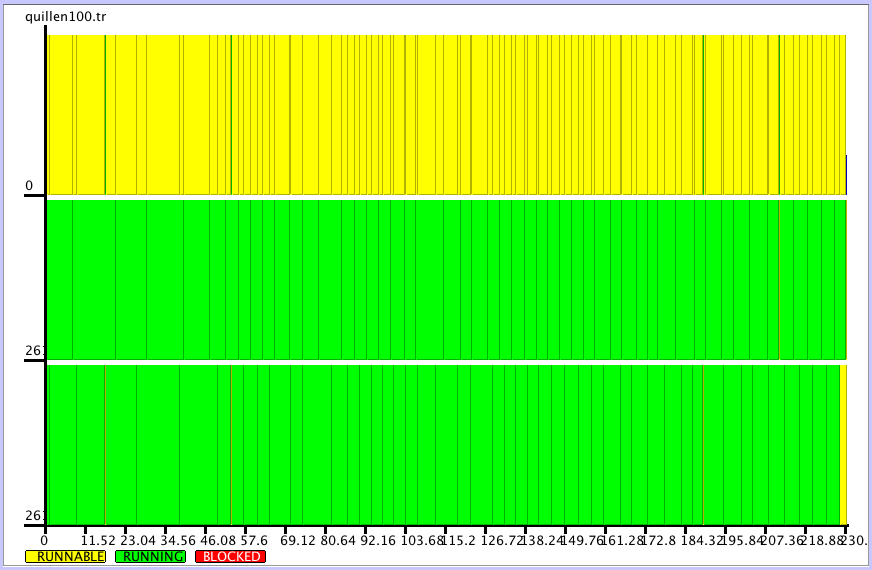
\includegraphics{img/quillen.pdf}}}  \vspace{10pt}\centerline{\resizebox{150mm}{!}{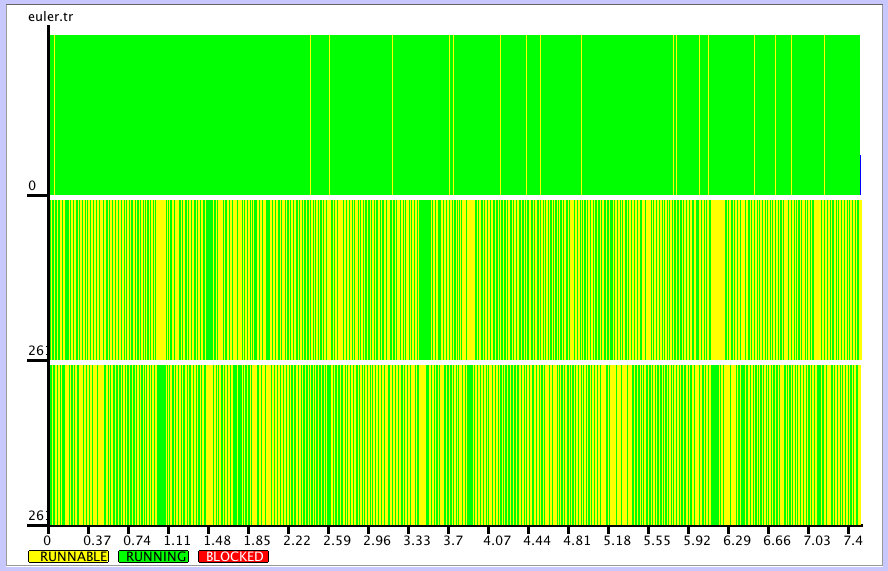
\includegraphics{img/euler.pdf}}}   The diagrams (made on an dual core MacBook laptop), shows that in the first
case parallelising is efficient and master successfully distributes load to
workers, while in the second case a single computation is just too short, so
most of the time is spent on communication. To parallelize the Euler's
function example efficiently, tasks must rather be grouped in chunks, which
should be enough large to reduce the communication overload, but enough small
to ensure that tasks are evenly distributed. 

 Of course, tracing can be used to investigate communication between a client
and a single server in a non-parallel context as well. For this purpose, \texttt{SCSCPservers} (\ref{SCSCPservers}) must be modified to contain only one server. }

 \texttt{ParListWithSCSCP} (\ref{ParListWithSCSCP}) can be easily modified to have parallel versions of other list operations like \texttt{ForAll} (\textbf{Reference: ForAll}), \texttt{ForAny} (\textbf{Reference: ForAny}), \texttt{First} (\textbf{Reference: First}), \texttt{Number} (\textbf{Reference: Number}), \texttt{Filtered} (\textbf{Reference: Filtered}), and also to have the skeleton in which the queue may be modified during the
computation (for example, to compute orbits). We plan to provide such tools in
one of the next versions of the package. }

 
\section{\textcolor{Chapter }{Example: parallelising Karatsuba multiplication for polynomials}}\label{Karatsuba}
\logpage{[ 8, 3, 0 ]}
\hyperdef{L}{X78C5AEA07F961325}{}
{
  The file \texttt{scscp/example/karatsuba.g} contains an implementation of the Karatsuba multiplication algorithm for
polynomials. This algorithm can be easily parallelized since each recursive
step creates three recursive calls of the same function for other polynomials. \emph{We will not parallelize each} recursive call, since this will create enormous data flow. Instead of this we
parallelize only the top-level function. For our experiments with
parallelising Karatsuba multiplication for polynomials with integer
coefficients we used the multi-core workstation, on which we started one \textsf{SCSCP} client and two \textsf{SCSCP} servers. To use it, modify the server configuration file adding to it the
command to read the file \texttt{scscp/example/karatsuba.g}, then define there the following function 
\begin{Verbatim}[commandchars=!@|,fontsize=\small,frame=single,label=Example]
  
  KaratsubaPolynomialMultiplicationExtRepByString:=function(s1,s2)
      return String( KaratsubaPolynomialMultiplicationExtRep( 
                     EvalString(s1), EvalString(s2) ) );
  end;;
  
\end{Verbatim}
 and finally add the following lines to made it available as an \textsf{SCSCP} procedure under the name \texttt{WS{\textunderscore}Karatsuba}: 
\begin{Verbatim}[commandchars=!@|,fontsize=\small,frame=single,label=Example]
  
  InstallSCSCPprocedure( "WS_Karatsuba", 
                         KaratsubaPolynomialMultiplicationExtRepByString);
  
\end{Verbatim}
 (we do not include it into the default \texttt{scscp/example/myserver.g} since the code contains a call to \texttt{EvalString} (\textbf{Reference: EvalString})). 

 This function provides a "bridge" between the client's function \texttt{KaratsubaPolynomialMultiplicationWS} and the server's function \texttt{KaratsubaPolynomialMultiplicationExtRep}, which performs the actual work on the server. \texttt{WS{\textunderscore}Karatsuba} converts its string arguments into internal representation of univariate
polynomials (basically, lists of integers) and then converts the result back
into string (since such data exchange format was chosen).  \newpage  We are going to parallelize the following part of the client's code: 
\begin{Verbatim}[commandchars=!@|,fontsize=\small,frame=single,label=Example]
  
  ...
  u := KaratsubaPolynomialMultiplicationExtRep(f1,g1);
  v := KaratsubaPolynomialMultiplicationExtRep(f0,g0);
  w := KaratsubaPolynomialMultiplicationExtRep(
         PlusLaurentPolynomialsExtRep(f1,f0),
         PlusLaurentPolynomialsExtRep(g1,g0) );
  ...
  
\end{Verbatim}
 and this can be done straightforwardly - we replace two first calls by calls
of the appropriate \textsf{SCSCP} services, then perform the 3rd call locally and then collect the results from
the two remote calls: 
\begin{Verbatim}[commandchars=!@|,fontsize=\small,frame=single,label=Example]
  
  ...
  u := NewProcess( "WS_Karatsuba",[ String(f1), String(g1) ],"localhost", 26133);   
  v := NewProcess( "WS_Karatsuba",[ String(f0), String(g0) ],"localhost", 26134);   
  w := KaratsubaPolynomialMultiplicationExtRep(
         PlusLaurentPolynomialsExtRep(f1,f0),
         PlusLaurentPolynomialsExtRep(g1,g0) );
  wsresult:=SynchronizeProcesses2( u,v );
  u := EvalString( wsresult[1].object );
  v := EvalString( wsresult[2].object );
  ...
  
\end{Verbatim}
 We obtain almost double speedup on three cores on randomly generated
polynomials of degree 32000: 
\begin{Verbatim}[commandchars=!@|,fontsize=\small,frame=single,label=Example]
  
  !gapprompt@gap>| !gapinput@ReadPackage("scscp/example/karatsuba.g");|
  !gapprompt@gap>| !gapinput@fam:=FamilyObj(1);;|
  !gapprompt@gap>| !gapinput@f:=LaurentPolynomialByCoefficients( fam, |
  !gapprompt@>| !gapinput@        List([1..32000],i->Random(Integers)), 0, 1 );;|
  !gapprompt@gap>| !gapinput@g:=LaurentPolynomialByCoefficients( fam, |
  !gapprompt@>| !gapinput@        List([1..32000],i->Random(Integers)), 0, 1 );;|
  !gapprompt@gap>| !gapinput@t2:=KaratsubaPolynomialMultiplication(f,g);;time;|
  5892
  !gapprompt@gap>| !gapinput@t3:=KaratsubaPolynomialMultiplicationWS(f,g);;time;|
  2974
  
\end{Verbatim}
 }

 }

 
\chapter{\textcolor{Chapter }{Service functions}}\label{Service}
\logpage{[ 9, 0, 0 ]}
\hyperdef{L}{X80DFB24F8289C323}{}
{
  
\section{\textcolor{Chapter }{Pinging \textsf{SCSCP} servers}}\label{Pinging}
\logpage{[ 9, 1, 0 ]}
\hyperdef{L}{X80F5FC948702D0F9}{}
{
  

\subsection{\textcolor{Chapter }{PingSCSCPservice}}
\logpage{[ 9, 1, 1 ]}\nobreak
\hyperdef{L}{X78B08D767F9ADB28}{}
{\noindent\textcolor{FuncColor}{$\triangleright$\ \ \texttt{PingSCSCPservice({\mdseries\slshape hostname, portnumber})\index{PingSCSCPservice@\texttt{PingSCSCPservice}}
\label{PingSCSCPservice}
}\hfill{\scriptsize (function)}}\\
\textbf{\indent Returns:\ }
 \texttt{true} or \texttt{fail} 



 This function returns \texttt{true} if the client can establish connection with the SCSCP server at \mbox{\texttt{\mdseries\slshape hostname}}:\mbox{\texttt{\mdseries\slshape portnumber}}. Otherwise, it returns \texttt{fail}. 
\begin{Verbatim}[commandchars=!@|,fontsize=\small,frame=single,label=Example]
  
  !gapprompt@gap>| !gapinput@PingSCSCPservice("localhost",26133);|
  true
  !gapprompt@gap>| !gapinput@PingSCSCPservice("localhost",26140);                     |
  Error: rec(
    message := "Connection refused",
    number := 61 )
  fail
  
\end{Verbatim}
 }

 

\subsection{\textcolor{Chapter }{PingStatistic}}
\logpage{[ 9, 1, 2 ]}\nobreak
\hyperdef{L}{X8345DE358064674E}{}
{\noindent\textcolor{FuncColor}{$\triangleright$\ \ \texttt{PingStatistic({\mdseries\slshape hostname, portnumber, n})\index{PingStatistic@\texttt{PingStatistic}}
\label{PingStatistic}
}\hfill{\scriptsize (function)}}\\
\textbf{\indent Returns:\ }
 nothing 



 The function is similar to the UNIX \texttt{ping}. It tries \mbox{\texttt{\mdseries\slshape n}} times to establish connection with the SCSCP server at \mbox{\texttt{\mdseries\slshape hostname}}:\mbox{\texttt{\mdseries\slshape portnumber}}, and then displays statistical information. 
\begin{Verbatim}[commandchars=!@|,fontsize=\small,frame=single,label=Example]
  
  !gapprompt@gap>| !gapinput@PingStatistic("localhost",26133,1000);|
  1000 packets transmitted, 1000 received, 0% packet loss, time 208ms
  min/avg/max = [ 0, 26/125, 6 ]
  
\end{Verbatim}
 }

 }

 
\section{\textcolor{Chapter }{Info classes for \textsf{SCSCP}}}\label{InfoClassesForSCSCP}
\logpage{[ 9, 2, 0 ]}
\hyperdef{L}{X7B232ED07F14DE80}{}
{
  

\subsection{\textcolor{Chapter }{InfoSCSCP}}
\logpage{[ 9, 2, 1 ]}\nobreak
\hyperdef{L}{X831E6A5D8695A3F9}{}
{\noindent\textcolor{FuncColor}{$\triangleright$\ \ \texttt{InfoSCSCP\index{InfoSCSCP@\texttt{InfoSCSCP}}
\label{InfoSCSCP}
}\hfill{\scriptsize (info class)}}\\


 \texttt{InfoSCSCP} is a special Info class for the \textsf{SCSCP} package. The amount of information to be displayed can be specified by the
user by setting InfoLevel for this class from 0 to 4, and the default value of
InfoLevel for the package is specified in the file \texttt{scscp/config.g}. The higher the level is, the more information will be displayed. To change
the InfoLevel to \texttt{k}, use the command \texttt{SetInfoLevel(InfoSCSCP, k)}. In the following examples we demonstrate various degrees of output details
using Info messages. 

 Default Info level: 
\begin{Verbatim}[commandchars=!@|,fontsize=\small,frame=single,label=Example]
  
  !gapprompt@gap>| !gapinput@SetInfoLevel(InfoSCSCP,2);                              |
  !gapprompt@gap>| !gapinput@EvaluateBySCSCP( "WS_Factorial",[10],"localhost",26133); |
  #I  Creating a socket ...
  #I  Connecting to a remote socket via TCP/IP ...
  #I  Got connection initiation message
  #I  <?scscp service_name="GAP" service_version="4.dev" service_id="localhost:2\
  6133:286" scscp_versions="1.0 1.1 1.2 1.3" ?>
  #I  Requesting version 1.3 from the server ...
  #I  Server confirmed version 1.3 to the client ...
  #I  Request sent ...
  #I  Waiting for reply ...
  #I  <?scscp start ?>
  #I  <?scscp end ?>
  #I  Got back: object 3628800 with attributes 
  [ [ "call_id", "localhost:26133:286:JL6KRQeh" ] ]
  rec( attributes := [ [ "call_id", "localhost:26133:286:JL6KRQeh" ] ], 
    object := 3628800 )
  
\end{Verbatim}
 

 Minimal Info level: 
\begin{Verbatim}[commandchars=!@|,fontsize=\small,frame=single,label=Example]
  
  !gapprompt@gap>| !gapinput@SetInfoLevel(InfoSCSCP,0);                              |
  !gapprompt@gap>| !gapinput@EvaluateBySCSCP( "WS_Factorial",[10],"localhost",26133);|
  rec( attributes := [ [ "call_id", "localhost:26133:286:jzjsp6th" ] ], 
    object := 3628800 )
  
\end{Verbatim}
 

 Verbose Info level: 
\begin{Verbatim}[commandchars=!@|,fontsize=\small,frame=single,label=Example]
  
  !gapprompt@gap>| !gapinput@SetInfoLevel(InfoSCSCP,3);|
  !gapprompt@gap>| !gapinput@EvaluateBySCSCP( "WS_Factorial",[10],"localhost",26133);|
  #I  Creating a socket ...
  #I  Connecting to a remote socket via TCP/IP ...
  #I  Got connection initiation message
  #I  <?scscp service_name="GAP" service_version="4.dev" service_id="localhost:2\
  6133:286" scscp_versions="1.0 1.1 1.2 1.3" ?>
  #I  Requesting version 1.3 from the server ...
  #I  Server confirmed version 1.3 to the client ...
  #I  Composing procedure_call message: 
  <?scscp start ?>
  <OMOBJ>
  	<OMATTR>
  		<OMATP>
  			<OMS cd="scscp1" name="call_id"/>
  			<OMSTR>localhost:26133:286:Jok6cQAf</OMSTR>
  			<OMS cd="scscp1" name="option_return_object"/>
  			<OMSTR></OMSTR>
  		</OMATP>
  		<OMA>
  			<OMS cd="scscp1" name="procedure_call"/>
  			<OMA>
  				<OMS cd="scscp_transient_1" name="WS_Factorial"/>
  				<OMI>10</OMI>
  			</OMA>
  		</OMA>
  	</OMATTR>
  </OMOBJ>
  <?scscp end ?>
  #I  Total length 396 characters 
  #I  Request sent ...
  #I  Waiting for reply ...
  #I  <?scscp start ?>
  #I Received message: 
  <OMOBJ>
  	<OMATTR>
  		<OMATP>
  			<OMS cd="scscp1" name="call_id"/>
  			<OMSTR>localhost:26133:286:Jok6cQAf</OMSTR>
  		</OMATP>
  		<OMA>
  			<OMS cd="scscp1" name="procedure_completed"/>
  			<OMI>3628800</OMI>
  		</OMA>
  	</OMATTR>
  </OMOBJ>
  #I  <?scscp end ?>
  #I  Got back: object 3628800 with attributes 
  [ [ "call_id", "localhost:26133:286:Jok6cQAf" ] ]
  rec( attributes := [ [ "call_id", "localhost:26133:286:Jok6cQAf" ] ], 
    object := 3628800 )
  !gapprompt@gap>| !gapinput@SetInfoLevel(InfoSCSCP,0);|
  
\end{Verbatim}
 }

 

\subsection{\textcolor{Chapter }{InfoMasterWorker}}
\logpage{[ 9, 2, 2 ]}\nobreak
\hyperdef{L}{X82AC628D7880D043}{}
{\noindent\textcolor{FuncColor}{$\triangleright$\ \ \texttt{InfoMasterWorker\index{InfoMasterWorker@\texttt{InfoMasterWorker}}
\label{InfoMasterWorker}
}\hfill{\scriptsize (info class)}}\\


 \texttt{InfoMasterWorker} is a special Info class for the Master-Worker skeleton \texttt{ParListWithSCSCP} (\ref{ParListWithSCSCP}). The amount of information to be displayed can be specified by the user by
setting InfoLevel for this class from 0 to 5, and the default value of
InfoLevel for the package is specified in the file \texttt{scscp/config.g}. The higher the level is, the more information will be displayed. To change
the InfoLevel to \texttt{k}, use the command \texttt{SetInfoLevel(InfoMasterWorker, k)}. In the following examples we demonstrate various degrees of output details
using Info messages. 

 Default Info level: 
\begin{Verbatim}[commandchars=!@|,fontsize=\small,frame=single,label=Example]
  
  !gapprompt@gap>| !gapinput@SetInfoLevel(InfoMasterWorker,2);|
  !gapprompt@gap>| !gapinput@ParListWithSCSCP( List( [2..6], n -> SymmetricGroup(n)), "WS_IdGroup" );|
  #I  1/5:master --> localhost:26133
  #I  2/5:master --> localhost:26134
  #I  3/5:master --> localhost:26133
  #I  4/5:master --> localhost:26134
  #I  5/5:master --> localhost:26133
  [ [ 2, 1 ], [ 6, 1 ], [ 24, 12 ], [ 120, 34 ], [ 720, 763 ] ]
  
\end{Verbatim}
 

 Minimal Info level: 
\begin{Verbatim}[commandchars=!@|,fontsize=\small,frame=single,label=Example]
  
  !gapprompt@gap>| !gapinput@SetInfoLevel(InfoSCSCP,0);       |
  !gapprompt@gap>| !gapinput@SetInfoLevel(InfoMasterWorker,0);|
  !gapprompt@gap>| !gapinput@ParListWithSCSCP( List( [2..6], n -> SymmetricGroup(n)), "WS_IdGroup" );|
  [ [ 2, 1 ], [ 6, 1 ], [ 24, 12 ], [ 120, 34 ], [ 720, 763 ] ]
  
\end{Verbatim}
 

 Verbose Info level: 
\begin{Verbatim}[commandchars=!@|,fontsize=\small,frame=single,label=Example]
  
  !gapprompt@gap>| !gapinput@SetInfoLevel(InfoMasterWorker,5);                                       |
  !gapprompt@gap>| !gapinput@ParListWithSCSCP( List( [2..6], n -> SymmetricGroup(n)), "WS_IdGroup" );|
  #I  1/5:master --> localhost:26133 : SymmetricGroup( [ 1 .. 2 ] )
  #I  2/5:master --> localhost:26134 : SymmetricGroup( [ 1 .. 3 ] )
  #I  localhost:26133 --> 1/5:master : [ 2, 1 ]
  #I  3/5:master --> localhost:26133 : SymmetricGroup( [ 1 .. 4 ] )
  #I  localhost:26134 --> 2/5:master : [ 6, 1 ]
  #I  4/5:master --> localhost:26134 : SymmetricGroup( [ 1 .. 5 ] )
  #I  localhost:26133 --> 3/5:master : [ 24, 12 ]
  #I  5/5:master --> localhost:26133 : SymmetricGroup( [ 1 .. 6 ] )
  #I  localhost:26134 --> 4/5:master : [ 120, 34 ]
  #I  localhost:26133 --> 5/5:master : [ 720, 763 ]
  [ [ 2, 1 ], [ 6, 1 ], [ 24, 12 ], [ 120, 34 ], [ 720, 763 ] ]
  !gapprompt@gap>| !gapinput@SetInfoLevel(InfoMasterWorker,2);|
  
\end{Verbatim}
 }

 }

 
\section{\textcolor{Chapter }{Other \textsf{SCSCP} Utilities}}\label{OtherSCSCPUtilities}
\logpage{[ 9, 3, 0 ]}
\hyperdef{L}{X7F9A75B381AE905D}{}
{
  

\subsection{\textcolor{Chapter }{DateISO8601}}
\logpage{[ 9, 3, 1 ]}\nobreak
\hyperdef{L}{X845DFBDA83AEF6B0}{}
{\noindent\textcolor{FuncColor}{$\triangleright$\ \ \texttt{DateISO8601({\mdseries\slshape })\index{DateISO8601@\texttt{DateISO8601}}
\label{DateISO8601}
}\hfill{\scriptsize (function)}}\\
\textbf{\indent Returns:\ }
 string 



 Returns the current date in the ISO-8601 YYYY-MM-DD format. This is an
internal function of the package which is used by the \textsf{SCSCP} server to generate the transient content dictionary, accordingly to the
definition of the \textsf{OpenMath} symbol \texttt{meta.CDDate}. 
\begin{Verbatim}[commandchars=!@|,fontsize=\small,frame=single,label=Example]
  
  !gapprompt@gap>| !gapinput@DateISO8601();|
  "2011-10-05"
  
\end{Verbatim}
 }

 

\subsection{\textcolor{Chapter }{CurrentTimestamp}}
\logpage{[ 9, 3, 2 ]}\nobreak
\hyperdef{L}{X79CE2568789D17D6}{}
{\noindent\textcolor{FuncColor}{$\triangleright$\ \ \texttt{CurrentTimestamp({\mdseries\slshape })\index{CurrentTimestamp@\texttt{CurrentTimestamp}}
\label{CurrentTimestamp}
}\hfill{\scriptsize (function)}}\\
\textbf{\indent Returns:\ }
 string 



 Returns the result of the call to \texttt{date}. This is an internal function of the package which is used to add the
timestamp to the \textsf{SCSCP} service description. 
\begin{Verbatim}[commandchars=!@|,fontsize=\small,frame=single,label=Example]
  
  !gapprompt@gap>| !gapinput@CurrentTimestamp();|
  "Tue 30 Mar 2010 11:19:38 BST"
  
\end{Verbatim}
 }

 

\subsection{\textcolor{Chapter }{Hostname}}
\logpage{[ 9, 3, 3 ]}\nobreak
\hyperdef{L}{X83A08C8883E5D3E1}{}
{\noindent\textcolor{FuncColor}{$\triangleright$\ \ \texttt{Hostname({\mdseries\slshape })\index{Hostname@\texttt{Hostname}}
\label{Hostname}
}\hfill{\scriptsize (function)}}\\
\textbf{\indent Returns:\ }
 string 



 Returns the result of the call to \texttt{hostname}. This function may be used in the configuration file \texttt{scscp/config.g} to specify that the default hostname which will be used by the \textsf{SCSCP} server will be detected automatically using \texttt{hostname}. 
\begin{Verbatim}[commandchars=!@|,fontsize=\small,frame=single,label=Example]
  
  !gapprompt@gap>| !gapinput@Hostname();|
  "scscp.symbolic-computing.co.uk"
  
\end{Verbatim}
 }

 

\subsection{\textcolor{Chapter }{MemoryUsageByGAPinKbytes}}
\logpage{[ 9, 3, 4 ]}\nobreak
\hyperdef{L}{X8312112E79686EF6}{}
{\noindent\textcolor{FuncColor}{$\triangleright$\ \ \texttt{MemoryUsageByGAPinKbytes({\mdseries\slshape })\index{MemoryUsageByGAPinKbytes@\texttt{MemoryUsageByGAPinKbytes}}
\label{MemoryUsageByGAPinKbytes}
}\hfill{\scriptsize (function)}}\\
\textbf{\indent Returns:\ }
 integer 



 Returns the current volume of the memory used by \textsf{GAP} in kylobytes. This is equivalent to calling \texttt{ps -p {\textless}PID{\textgreater} -o vsz}, where \texttt{{\textless}PID{\textgreater}} is the process ID of the \textsf{GAP} process. This is an internal function of the package which is used by the \textsf{SCSCP} server to report its memory usage in the \texttt{info{\textunderscore}memory} attribute when being called with the option \texttt{debuglevel=2} (see options in \texttt{EvaluateBySCSCP} (\ref{EvaluateBySCSCP}) and \texttt{NewProcess} (\ref{NewProcess})). 
\begin{Verbatim}[commandchars=!@|,fontsize=\small,frame=single,label=Example]
  
  !gapprompt@gap>| !gapinput@MemoryUsageByGAPinKbytes();|
  649848
  
\end{Verbatim}
 }

 

\subsection{\textcolor{Chapter }{LastReceivedCallID}}
\logpage{[ 9, 3, 5 ]}\nobreak
\hyperdef{L}{X844EC26F84D921CE}{}
{\noindent\textcolor{FuncColor}{$\triangleright$\ \ \texttt{LastReceivedCallID({\mdseries\slshape })\index{LastReceivedCallID@\texttt{LastReceivedCallID}}
\label{LastReceivedCallID}
}\hfill{\scriptsize (function)}}\\
\textbf{\indent Returns:\ }
 string 



 Returns the call ID contained in the most recently received message. It may
contain some useful debugging information; in particular, the call ID for the \textsf{GAP} \textsf{SCSCP} client and server contains colon-separated server name, port number, process
ID and a random string. 
\begin{Verbatim}[commandchars=!@|,fontsize=\small,frame=single,label=Example]
  
  !gapprompt@gap>| !gapinput@LastReceivedCallID();|
  "scscp.symbolic-computing.co.uk:26133:77372:choDZBgA"
  
\end{Verbatim}
 }

 

\subsection{\textcolor{Chapter }{IO{\textunderscore}PickleToString}}
\logpage{[ 9, 3, 6 ]}\nobreak
\hyperdef{L}{X84F055ED860120D5}{}
{\noindent\textcolor{FuncColor}{$\triangleright$\ \ \texttt{IO{\textunderscore}PickleToString({\mdseries\slshape obj})\index{IOPickleToString@\texttt{IO{\textunderscore}PickleToString}}
\label{IOPickleToString}
}\hfill{\scriptsize (function)}}\\
\textbf{\indent Returns:\ }
 string containing "pickled" object 



 This function "pickles" or "serialises" the object \mbox{\texttt{\mdseries\slshape obj}} using the operation \texttt{IO{\textunderscore}Pickle} (\textbf{IO: IO{\textunderscore}Pickle}) from the \textsf{IO} package, and writes it to a string, from which it could be later restored
using \texttt{IO{\textunderscore}UnpickleFromString} (\ref{IOUnpickleFromString}). This provides a way to design \textsf{SCSCP} procedures which transmit \textsf{GAP} objects in the "pickled" format as \textsf{OpenMath} strings, which may be useful for objects which may be "pickled" by the \textsf{IO} package but can not be converted to \textsf{OpenMath} or for which the "pickled" representation is more compact or can be
encoded/decoded much faster. 

 See \texttt{IO{\textunderscore}Pickle} (\textbf{IO: IO{\textunderscore}Pickle}) and \texttt{IO{\textunderscore}Unpickle} (\textbf{IO: IO{\textunderscore}Unpickle}) for more details. 
\begin{Verbatim}[commandchars=!@|,fontsize=\small,frame=single,label=Example]
  
  !gapprompt@gap>| !gapinput@f := IO_PickleToString( GF( 125 ) );|
  "FFIEINTG\>15INTG\>13FAIL"
  
\end{Verbatim}
 }

 

\subsection{\textcolor{Chapter }{IO{\textunderscore}UnpickleFromString}}
\logpage{[ 9, 3, 7 ]}\nobreak
\hyperdef{L}{X813EACD27C218E19}{}
{\noindent\textcolor{FuncColor}{$\triangleright$\ \ \texttt{IO{\textunderscore}UnpickleFromString({\mdseries\slshape s})\index{IOUnpickleFromString@\texttt{IO{\textunderscore}}\-\texttt{Unpickle}\-\texttt{From}\-\texttt{String}}
\label{IOUnpickleFromString}
}\hfill{\scriptsize (function)}}\\
\textbf{\indent Returns:\ }
 "unpickled" GAP object 



 This function "unpickles" the string \mbox{\texttt{\mdseries\slshape s}} which was created using the function \texttt{IO{\textunderscore}PickleToString} (\ref{IOPickleToString}), using the operation \texttt{IO{\textunderscore}Unpickle} (\textbf{IO: IO{\textunderscore}Unpickle}) from the \textsf{IO} package. See \texttt{IO{\textunderscore}PickleToString} (\ref{IOPickleToString}) for more details and suggestions about its usage. 
\begin{Verbatim}[commandchars=!@|,fontsize=\small,frame=single,label=Example]
  
  !gapprompt@gap>| !gapinput@IO_UnpickleFromString( f );                    |
  GF(5^3)
  !gapprompt@gap>| !gapinput@f = IO_UnpickleFromString( IO_PickleToString( f ) ); |
  true
  
\end{Verbatim}
 }

 }

 }

 \def\bibname{References\logpage{[ "Bib", 0, 0 ]}
\hyperdef{L}{X7A6F98FD85F02BFE}{}
}

\bibliographystyle{alpha}
\bibliography{manual}

\addcontentsline{toc}{chapter}{References}

\def\indexname{Index\logpage{[ "Ind", 0, 0 ]}
\hyperdef{L}{X83A0356F839C696F}{}
}

\cleardoublepage
\phantomsection
\addcontentsline{toc}{chapter}{Index}


\printindex

\newpage
\immediate\write\pagenrlog{["End"], \arabic{page}];}
\immediate\closeout\pagenrlog
\end{document}
